% Options for packages loaded elsewhere
\PassOptionsToPackage{unicode}{hyperref}
\PassOptionsToPackage{hyphens}{url}
\PassOptionsToPackage{dvipsnames,svgnames,x11names}{xcolor}
%
\documentclass[
  10pt,
  a4paper]{article}
\usepackage{amsmath,amssymb}
\usepackage{iftex}
\ifPDFTeX
  \usepackage[T1]{fontenc}
  \usepackage[utf8]{inputenc}
  \usepackage{textcomp} % provide euro and other symbols
\else % if luatex or xetex
  \usepackage{unicode-math} % this also loads fontspec
  \defaultfontfeatures{Scale=MatchLowercase}
  \defaultfontfeatures[\rmfamily]{Ligatures=TeX,Scale=1}
\fi
\usepackage{lmodern}
\ifPDFTeX\else
  % xetex/luatex font selection
\fi
% Use upquote if available, for straight quotes in verbatim environments
\IfFileExists{upquote.sty}{\usepackage{upquote}}{}
\IfFileExists{microtype.sty}{% use microtype if available
  \usepackage[]{microtype}
  \UseMicrotypeSet[protrusion]{basicmath} % disable protrusion for tt fonts
}{}
\makeatletter
\@ifundefined{KOMAClassName}{% if non-KOMA class
  \IfFileExists{parskip.sty}{%
    \usepackage{parskip}
  }{% else
    \setlength{\parindent}{0pt}
    \setlength{\parskip}{6pt plus 2pt minus 1pt}}
}{% if KOMA class
  \KOMAoptions{parskip=half}}
\makeatother
\usepackage{xcolor}
\usepackage[margin=2.2cm]{geometry}
\usepackage{longtable,booktabs,array}
\usepackage{calc} % for calculating minipage widths
% Correct order of tables after \paragraph or \subparagraph
\usepackage{etoolbox}
\makeatletter
\patchcmd\longtable{\par}{\if@noskipsec\mbox{}\fi\par}{}{}
\makeatother
% Allow footnotes in longtable head/foot
\IfFileExists{footnotehyper.sty}{\usepackage{footnotehyper}}{\usepackage{footnote}}
\makesavenoteenv{longtable}
\usepackage{graphicx}
\makeatletter
\def\maxwidth{\ifdim\Gin@nat@width>\linewidth\linewidth\else\Gin@nat@width\fi}
\def\maxheight{\ifdim\Gin@nat@height>\textheight\textheight\else\Gin@nat@height\fi}
\makeatother
% Scale images if necessary, so that they will not overflow the page
% margins by default, and it is still possible to overwrite the defaults
% using explicit options in \includegraphics[width, height, ...]{}
\setkeys{Gin}{width=\maxwidth,height=\maxheight,keepaspectratio}
% Set default figure placement to htbp
\makeatletter
\def\fps@figure{htbp}
\makeatother
\setlength{\emergencystretch}{3em} % prevent overfull lines
\providecommand{\tightlist}{%
  \setlength{\itemsep}{0pt}\setlength{\parskip}{0pt}}
\setcounter{secnumdepth}{-\maxdimen} % remove section numbering
\usepackage{float}
\floatplacement{figure}{H}
\usepackage{newunicodechar}
\newunicodechar{₂}{\textsubscript{2}}
\newunicodechar{≥}{\ensuremath{\geq}}
\newunicodechar{≤}{\ensuremath{\leq}}
\newunicodechar{×}{\ensuremath{\times}}
\newunicodechar{→}{\ensuremath{\rightarrow}}
\newunicodechar{≈}{\ensuremath{\approx}}
\newunicodechar{±}{\ensuremath{\pm}}
\newunicodechar{°}{\ensuremath{^\circ}}
\newunicodechar{µ}{\ensuremath{\mu}}
\newunicodechar{−}{\ensuremath{-}}
\newunicodechar{万}{wan}
\ifLuaTeX
  \usepackage{selnolig}  % disable illegal ligatures
\fi
\IfFileExists{bookmark.sty}{\usepackage{bookmark}}{\usepackage{hyperref}}
\IfFileExists{xurl.sty}{\usepackage{xurl}}{} % add URL line breaks if available
\urlstyle{same}
\hypersetup{
  pdftitle={OrbitCu: Satellite Monitoring of the Largest Copper Smelters},
  pdfauthor={Baptiste, Radu, Ethan, Robin --- Group CoPPernicus, CSE 406 Software Engineering},
  colorlinks=true,
  linkcolor={Maroon},
  filecolor={Maroon},
  citecolor={Blue},
  urlcolor={Blue},
  pdfcreator={LaTeX via pandoc}}

\title{OrbitCu: Satellite Monitoring of the Largest Copper Smelters}
\usepackage{etoolbox}
\makeatletter
\providecommand{\subtitle}[1]{% add subtitle to \maketitle
  \apptocmd{\@title}{\par {\large #1 \par}}{}{}
}
\makeatother
\subtitle{Proposal, Requirements and Technical Report}
\author{Baptiste, Radu, Ethan, Robin --- Group CoPPernicus, CSE 406
Software Engineering}
\date{November 2026}

\begin{document}
\maketitle

{
\hypersetup{linkcolor=}
\setcounter{tocdepth}{2}
\tableofcontents
}
\textbf{\emph{Abstract---}Copper is a strategic metal for
electrification, yet official statistics on refined copper output are
published weeks after the fact, and the commercial satellite services
that track smelters are closed and expensive. We propose OrbitCu, an
open, reproducible big-data system that measures, every day, whether the
30 largest copper smelters in the world are operating. The system
ingests several terabytes of free Earth-observation data (Sentinel-2 and
Landsat shortwave-infrared imagery, VIIRS night-time thermal detections,
Sentinel-5P sulfur dioxide columns and ERA5 winds), detects furnace heat
and SO₂ emissions at each site, fuses these heterogeneous signals in a
state-space model, and publishes capacity-weighted global and regional
activity indices. These indices are validated against known events and
official production data, used to nowcast monthly refined output, and
evaluated in a rigorous point-in-time backtest of copper futures
strategies. The whole pipeline runs on Kubernetes with event-driven,
autoscaled workflows, a lakehouse storage layer, experiment tracking and
a web dashboard. This document presents the motivation, related work and
the functional requirements of the system.}

\textbf{\emph{Index Terms---}big data pipeline, Kubernetes, remote
sensing, Sentinel-2, Sentinel-5P, copper, commodity trading, nowcasting,
MLOps.}

\part{Proposal and Requirements}

\textsc{Table I}

\textsc{Role Assignments (Until Mid-Term)}

\begin{longtable}[]{@{}
  >{\raggedright\arraybackslash}p{(\columnwidth - 6\tabcolsep) * \real{0.2400}}
  >{\raggedright\arraybackslash}p{(\columnwidth - 6\tabcolsep) * \real{0.1600}}
  >{\raggedright\arraybackslash}p{(\columnwidth - 6\tabcolsep) * \real{0.3333}}
  >{\raggedright\arraybackslash}p{(\columnwidth - 6\tabcolsep) * \real{0.2400}}@{}}
\toprule\noalign{}
\begin{minipage}[b]{\linewidth}\raggedright
\textbf{Role}
\end{minipage} & \begin{minipage}[b]{\linewidth}\raggedright
\textbf{Name}
\end{minipage} & \begin{minipage}[b]{\linewidth}\raggedright
\textbf{Responsibilities (role)}
\end{minipage} & \begin{minipage}[b]{\linewidth}\raggedright
\textbf{Technical module owned}
\end{minipage} \\
\midrule\noalign{}
\endhead
\bottomrule\noalign{}
\endlastfoot
\textbf{User} & Robin & Speaks for the analyst/trader: writes use cases,
tests the dashboard and signals. & Market data, nowcast, backtest,
dashboard \\
\textbf{Customer} & Ethan & Speaks for the trading desk: sets and
prioritizes requirements, accepts deliverables. & SO₂ estimation,
fusion, activity indices \\
\textbf{Software developer} & Radu & Maintains code standards:
structure, reviews, testing rules. & Satellite ingestion, thermal
detection \\
\textbf{Development manager} & Baptiste & Coordinates the team process:
shared schedule, weekly meetings, integration, decision log. &
Kubernetes, CI/CD, smelter registry, data contracts \\
\end{longtable}

Each member holds one role until mid-term and develops one module. The
team has no leader: decisions are taken collectively at the weekly
meeting.

\hypertarget{i.-introduction}{%
\section{I. Introduction}\label{i.-introduction}}

\hypertarget{a.-motivation}{%
\subsection{A. Motivation}\label{a.-motivation}}

Copper is essential to power grids, electric vehicles and renewable
energy, which makes its supply a central question for producers,
consumers and traders. Mined concentrate must be processed in smelters
before it becomes refined metal, and a relatively small number of large
smelters accounts for most of the world's capacity. When a major smelter
stops for maintenance, an accident or a power shortage, refined supply
tightens, inventories react, and futures prices and spreads can move.

Market participants, however, learn about these changes late. Official
production statistics are released monthly, typically weeks after the
end of the month, and company disclosures are irregular. Smelters, on
the other hand, leave physical traces that are visible from space:
furnaces and converters emit intense heat detectable in
shortwave-infrared imagery, and the smelting of sulfide ores releases
sulfur dioxide measurable by atmospheric sensors. Free satellite
missions now observe the whole planet every few days, which makes it
possible to build an objective, near-real-time measure of smelting
activity.

\hypertarget{b.-problem-statement-and-client-needs}{%
\subsection{B. Problem Statement and Client
Needs}\label{b.-problem-statement-and-client-needs}}

Our client is a commodity trading or research desk that needs a timely
and verifiable view of refined copper supply. Its needs are the
following:

\begin{quote}
-- \emph{Timeliness:} an estimate of smelter activity days or weeks
before official data.

-- \emph{Transparency:} a method whose every number can be traced back
to raw observations, unlike black-box commercial products.

-- \emph{Point-in-time history:} a history that records when each piece
of information became available, so that trading strategies can be
backtested without look-ahead bias.

-- \emph{Actionability:} nowcasts of official production and an honest
evaluation of whether the signal improves copper futures strategies.

-- \emph{Affordability:} a solution built on free data and open-source
software.
\end{quote}

Meeting these needs requires processing several terabytes of
heterogeneous geospatial data reliably and repeatedly, which motivates a
scalable, Kubernetes-based data pipeline.

\hypertarget{c.-related-software-and-research}{%
\subsection{C. Related Software and
Research}\label{c.-related-software-and-research}}

Two kinds of existing work are relevant: commercial services that
already sell satellite smelter data, which prove the signal has value,
and research tools that provide technical building blocks. Table II
summarizes them.

\textsc{Table II}

\textsc{Related Software and Research}

\begin{longtable}[]{@{}
  >{\raggedright\arraybackslash}p{(\columnwidth - 4\tabcolsep) * \real{0.2667}}
  >{\raggedright\arraybackslash}p{(\columnwidth - 4\tabcolsep) * \real{0.4000}}
  >{\raggedright\arraybackslash}p{(\columnwidth - 4\tabcolsep) * \real{0.3067}}@{}}
\toprule\noalign{}
\begin{minipage}[b]{\linewidth}\raggedright
\textbf{Work}
\end{minipage} & \begin{minipage}[b]{\linewidth}\raggedright
\textbf{What it does}
\end{minipage} & \begin{minipage}[b]{\linewidth}\raggedright
\textbf{Limitation for our client}
\end{minipage} \\
\midrule\noalign{}
\endhead
\bottomrule\noalign{}
\endlastfoot
\textbf{SAVANT, Earth-i {[}1{]}--{[}3{]}} & Satellite monitoring of
copper smelters (about 70\% of world capacity), launched in 2019 with
the broker Marex & Closed and paid (\$10k--\$250k per year at launch) \\
\textbf{SMM {[}4{]}} & Relays satellite estimates of inactive capacity
(11.8\% in Aug.~2025) & Headline figures only \\
\textbf{TransitionZero, Climate TRACE {[}5{]}} & Infrared hotspots to
estimate the activity of heavy-industry sites & Not specific to
copper \\
\textbf{Massimetti et al. {[}6{]}} & Sentinel-2 shortwave-infrared
hotspot detection & Designed for volcanoes \\
\textbf{Fioletov et al. {[}7{]}} & Catalogue of 491 large SO₂ sources,
including 53 smelters & Annual emissions, not daily activity \\
\textbf{ddeq library {[}8{]}} & Open-source emission estimation for
point sources (e.g., flux divergence) & Demonstrated on NO₂, not SO₂ \\
\textbf{Finch and Palmer {[}9{]}} & U-Net detection of SO₂ plumes in
TROPOMI images & Detects plumes, not smelter activity; weaker in
China \\
\end{longtable}

\emph{Gap.} No open-source system combines these building blocks into an
end-to-end, reproducible copper smelter activity index and evaluates its
value for trading. OrbitCu aims to fill this gap.

\hypertarget{d.-proposed-solution-and-scope}{%
\subsection{D. Proposed Solution and
Scope}\label{d.-proposed-solution-and-scope}}

OrbitCu is organized as a pipeline of independent stages: (1) a smelter
registry; (2) satellite data ingestion; (3) thermal hotspot detection;
(4) SO₂ emission estimation; (5) multi-sensor fusion into a daily
operating state per site; (6) capacity-weighted activity indices; (7)
validation and production nowcasting; (8) point-in-time backtesting of
copper futures strategies; and (9) a web dashboard. All stages run as
containerized workflows on a Kubernetes cluster colocated with the
Microsoft Planetary Computer data catalogue {[}10{]}.

The system covers the 30 largest copper smelters in the world.
Real-money trading, commercial high-resolution imagery and copper mine
monitoring are out of scope.

\hypertarget{ii.-requirements}{%
\section{II. Requirements}\label{ii.-requirements}}

\textbf{1. Smelter registry.} The system shall maintain a versioned
catalogue of copper smelters (identifier, coordinates, area of interest,
capacity, owner). It is the single reference shared by all stages and
covers the 30 largest copper smelters.

\textbf{2. Satellite data ingestion.} The system shall ingest
Sentinel-2, Landsat 8/9, VIIRS, Sentinel-5P SO₂ and ERA5 wind data
through the Planetary Computer STAC API {[}10{]} and public APIs (e.g.,
NASA FIRMS for VIIRS), as a historical backfill (2018 to present) and
incrementally as new acquisitions are published.

\textbf{3. Site activity detection.} For each site and acquisition, the
system shall compute a thermal hotspot score from shortwave-infrared
bands and an SO₂ emission estimate from Sentinel-5P and ERA5 winds, each
with a cloud or quality flag.

\textbf{4. Fusion and activity indices.} The system shall fuse all
observations of a site into a daily probability of being active, robust
to cloud gaps, and publish capacity-weighted global and regional
activity indices.

\textbf{5. Validation.} The system shall compare site states and indices
with a catalogue of known events (shutdowns, start-ups), with official
production statistics and with publicly released SAVANT index figures,
and produce a validation report.

\textbf{6. Market data and nowcasting.} The system shall ingest copper
futures prices, exchange inventories and official production statistics
with their publication dates, and nowcast monthly refined production
before its release.

\textbf{7. Backtesting.} The system shall backtest copper futures
strategies driven by the indices, with walk-forward validation, contract
rolls and transaction costs, and report performance and risk metrics.

\textbf{8. Dashboard.} The system shall provide a web dashboard showing
a map of smelters and their status, site time series, indices, nowcasts
and backtest results.

\hypertarget{iii.-development-environment}{%
\section{III. Development
Environment}\label{iii.-development-environment}}

\hypertarget{a.-choice-of-software-development-platform}{%
\subsection{A. Choice of Software Development
Platform}\label{a.-choice-of-software-development-platform}}

\textbf{Platform.} OrbitCu is planned as a server-side data processing
pipeline with a web dashboard. Each step of the pipeline will be
packaged as a Linux container and run on a local Kubernetes setup, while
users view the results in a standard web browser with nothing to
install. Because our team uses Windows laptops, we plan to use WSL 2
(Windows Subsystem for Linux) and Docker Desktop during development so
that everyone works in the exact same environment.

We chose Linux containers and Kubernetes for three practical reasons.
First, many satellite and geospatial Python libraries (such as GDAL and
rasterio) are developed primarily on Linux and frequently cause
installation conflicts on Windows. Second, Docker containers make our
work reproducible: if a script works on one teammate\textquotesingle s
laptop, it will run the same way for the rest of the team. Third,
downloading and processing several years of satellite data for 30
smelters involves many repetitive tasks; a basic Kubernetes setup lets
us run these jobs automatically in parallel and retry them if a download
fails.

\textbf{Language.} We plan to use \textbf{Python 3.12} for the entire
pipeline, from downloading data to building the web dashboard, along
with basic SQL (via DuckDB) to query our saved data tables. Python is
the standard language for satellite data analysis, statistics, and
finance, so we can rely on existing open-source libraries rather than
writing custom tools from scratch. It is also the programming language
all four team members already know. For the web dashboard, we plan to
use Plotly Dash, which lets us build interactive web pages directly in
Python without needing a separate JavaScript front end.

\textbf{Cost estimation.} All satellite, weather, and market data
sources we plan to use are free for students and researchers, and every
software tool is open source. We will develop and test the project on
our own laptops, meaning the project requires no hardware or software
purchases. The only optional cost would be deploying the system on a
cloud server later in the semester using free student credits (Table
III).

\textsc{Table III}

\textsc{Cost Estimation (4-Month Project)}

\begin{longtable}[]{@{}
  >{\raggedright\arraybackslash}p{(\columnwidth - 4\tabcolsep) * \real{0.2785}}
  >{\raggedright\arraybackslash}p{(\columnwidth - 4\tabcolsep) * \real{0.4177}}
  >{\raggedright\arraybackslash}p{(\columnwidth - 4\tabcolsep) * \real{0.2785}}@{}}
\toprule\noalign{}
\begin{minipage}[b]{\linewidth}\raggedright
\textbf{Item}
\end{minipage} & \begin{minipage}[b]{\linewidth}\raggedright
\textbf{Planned Choice}
\end{minipage} & \begin{minipage}[b]{\linewidth}\raggedright
\textbf{Estimated Cost}
\end{minipage} \\
\midrule\noalign{}
\endhead
\bottomrule\noalign{}
\endlastfoot
Satellite and weather data & Microsoft Planetary Computer, NASA FIRMS,
Copernicus CDS (free APIs) & \$0 \\
Market data & LSEG Workspace (student access held by a team member) and
public reports & \$0 \\
Software & Python, Docker, kind (local Kubernetes), Argo, MLflow, Dash,
DuckDB (open source) & \$0 \\
Hardware & Team members\textquotesingle{} personal laptops & \$0 \\
Local Kubernetes cluster & kind (Kubernetes running locally inside
Docker Desktop) & \$0 \\
Cloud cluster (optional bonus) & Microsoft Azure (AKS) with basic
virtual machines and storage & \textasciitilde\$80--\$100/month \\
Cloud funding & Azure for Students credit (\$100 free credit per team
member) {[}11{]} & \$400 available \\
\end{longtable}

Cloud costs are rough estimates from Azure public pricing {[}12{]}.
Running locally on our laptops is completely free and is our primary
setup.

\textbf{Cloud deployment (optional bonus).} To avoid complex cloud setup
and avoid burning through our credits while we are still learning, we
will build and run the entire Kubernetes pipeline locally on our laptops
using \emph{kind} (Kubernetes in Docker). Because Microsoft hosts the
Planetary Computer satellite archive on Azure {[}10{]}, we may
optionally deploy our containers to Azure Kubernetes Service (AKS) at
the end of the project using our Azure for Students credits {[}11{]}.
However, the full system is designed to work locally for free.

\textbf{Planned development environment.} Table IV lists the software
tools and Python libraries we selected after researching online
documentation and similar satellite projects. Because we are at the
beginning of the project and have not started coding the modules yet, we
plan to install standard current versions of these libraries and lock
the exact version numbers once we set up our shared repository.

\textsc{Table IV}

Planned Development Environment

\begin{longtable}[]{@{}
  >{\raggedright\arraybackslash}p{(\columnwidth - 2\tabcolsep) * \real{0.3243}}
  >{\raggedright\arraybackslash}p{(\columnwidth - 2\tabcolsep) * \real{0.6486}}@{}}
\toprule\noalign{}
\begin{minipage}[b]{\linewidth}\raggedright
\textbf{Component}
\end{minipage} & \begin{minipage}[b]{\linewidth}\raggedright
\textbf{Planned Specification / Tools}
\end{minipage} \\
\midrule\noalign{}
\endhead
\bottomrule\noalign{}
\endlastfoot
Team laptops & Personal Windows 11 laptops (16--32 GB RAM) with WSL 2
(Ubuntu Linux) \\
Containers & Docker Desktop with standard Ubuntu Linux container
images \\
Programming language & Python 3.12 managed with Conda / virtual
environments \\
Editor and version control & Visual Studio Code, Git, and GitHub (shared
repository, pull requests, basic automated checks) \\
Satellite \& geospatial libraries & pystac-client, planetary-computer,
rasterio, shapely, xarray, cdsapi \\
Data tables \& storage & pandas, numpy, scipy, duckdb, and local Parquet
/ CSV files \\
Modeling \& tracking & scikit-learn, statsmodels, and MLflow (to save
model results) \\
Market data & LSEG Workspace Python library and downloaded CSV data
files \\
Dashboard & Plotly Dash and matplotlib \\
Container scheduling & Local Kubernetes (kind) and Argo Workflows (to
run pipeline steps in order) {[}13{]} \\
Testing & pytest for testing our Python functions \\
\end{longtable}

We plan to organize our GitHub repository with separate folders for each
stage of the pipeline (smelter list, data download, heat detection, gas
detection, sensor fusion, backtesting, and dashboard). Personal API keys
(such as NASA FIRMS and Copernicus tokens) will be stored in local
configuration files on our laptops and never uploaded to GitHub.

\hypertarget{b.-software-in-use}{%
\subsection{B. Software in Use}\label{b.-software-in-use}}

Instead of inventing our own satellite processing or financial formulas
from scratch, we plan to use existing public satellite datasets and
simplified versions of methods described in research papers. Table V
lists the reference systems and methods we found during our initial
research.

\textsc{Table V}

\textsc{Existing Software and Algorithms}

\begin{longtable}[]{@{}
  >{\raggedright\arraybackslash}p{(\columnwidth - 4\tabcolsep) * \real{0.2933}}
  >{\raggedright\arraybackslash}p{(\columnwidth - 4\tabcolsep) * \real{0.4133}}
  >{\raggedright\arraybackslash}p{(\columnwidth - 4\tabcolsep) * \real{0.2667}}@{}}
\toprule\noalign{}
\begin{minipage}[b]{\linewidth}\raggedright
\textbf{Software / method}
\end{minipage} & \begin{minipage}[b]{\linewidth}\raggedright
\textbf{How we plan to use it in OrbitCu}
\end{minipage} & \begin{minipage}[b]{\linewidth}\raggedright
\textbf{Reference}
\end{minipage} \\
\midrule\noalign{}
\endhead
\bottomrule\noalign{}
\endlastfoot
Earth-i SAVANT & Commercial copper smelter index; we will use their
public news figures as a reference check (Requirement 5) &
{[}1{]}--{[}4{]} \\
TransitionZero / Climate TRACE & Similar projects that monitor heavy
industry from space; used as inspiration for our project design &
{[}5{]} \\
NASA FIRMS VIIRS hotspots & Ready-to-use satellite table of night-time
heat hotspots and fire radiative power (FRP) & {[}14{]}, {[}15{]} \\
Sentinel-2 SWIR heat formula & Simple infrared band ratio from research
papers to spot hot smelter surfaces & {[}6{]} \\
Sentinel-5P (TROPOMI) SO₂ & Ready-to-use satellite product measuring
sulfur dioxide gas in the air with a quality score & {[}16{]} \\
Wind-rotated SO₂ \& ddeq library & Published method and open-source
Python package to estimate gas emissions using wind direction & {[}7{]},
{[}8{]} \\
Hidden Markov Model (HMM) & Basic statistical model to estimate whether
a smelter is ON or OFF each day from noisy data & {[}17{]} \\
Linear regression nowcasting & Predicting monthly copper production from
our daily satellite index using linear regression & {[}18{]} \\
Sharpe ratio \& backtest metrics & Standard finance metrics to evaluate
our trading simulation against a simple baseline & {[}19{]} \\
ERA5 weather data & Global weather dataset used to get wind speed and
direction around each smelter & {[}20{]} \\
\end{longtable}

\hypertarget{c.-task-distribution}{%
\subsection{C. Task Distribution}\label{c.-task-distribution}}

Until the mid-term evaluation, each team member is responsible for
researching and developing one main module as listed in Table I. We will
define the detailed coding tasks for each requirement during the
upcoming design phase.

\hypertarget{iv.-specifications}{%
\section{IV. Specifications}\label{iv.-specifications}}

This section explains how we plan to build each requirement from Section
II using the tools in Section III. Fig. 1 shows how the pipeline steps
connect. To keep our files organized and avoid confusion with copper, we
store data in three simple folders: \textbf{Raw Data} (cropped satellite
images and weather data as downloaded), \textbf{Processed Data} (clean
tables where each row stores the heat or gas score for one smelter on
one satellite pass), and \textbf{Final Outputs} (daily smelter ON/OFF
probabilities, regional activity indices, and financial results). Every
record saves both the date the satellite took the picture
(\emph{observation\_date}) and the date it was published online
(\emph{available\_date}), so our backtest only uses information that was
actually known on that day.

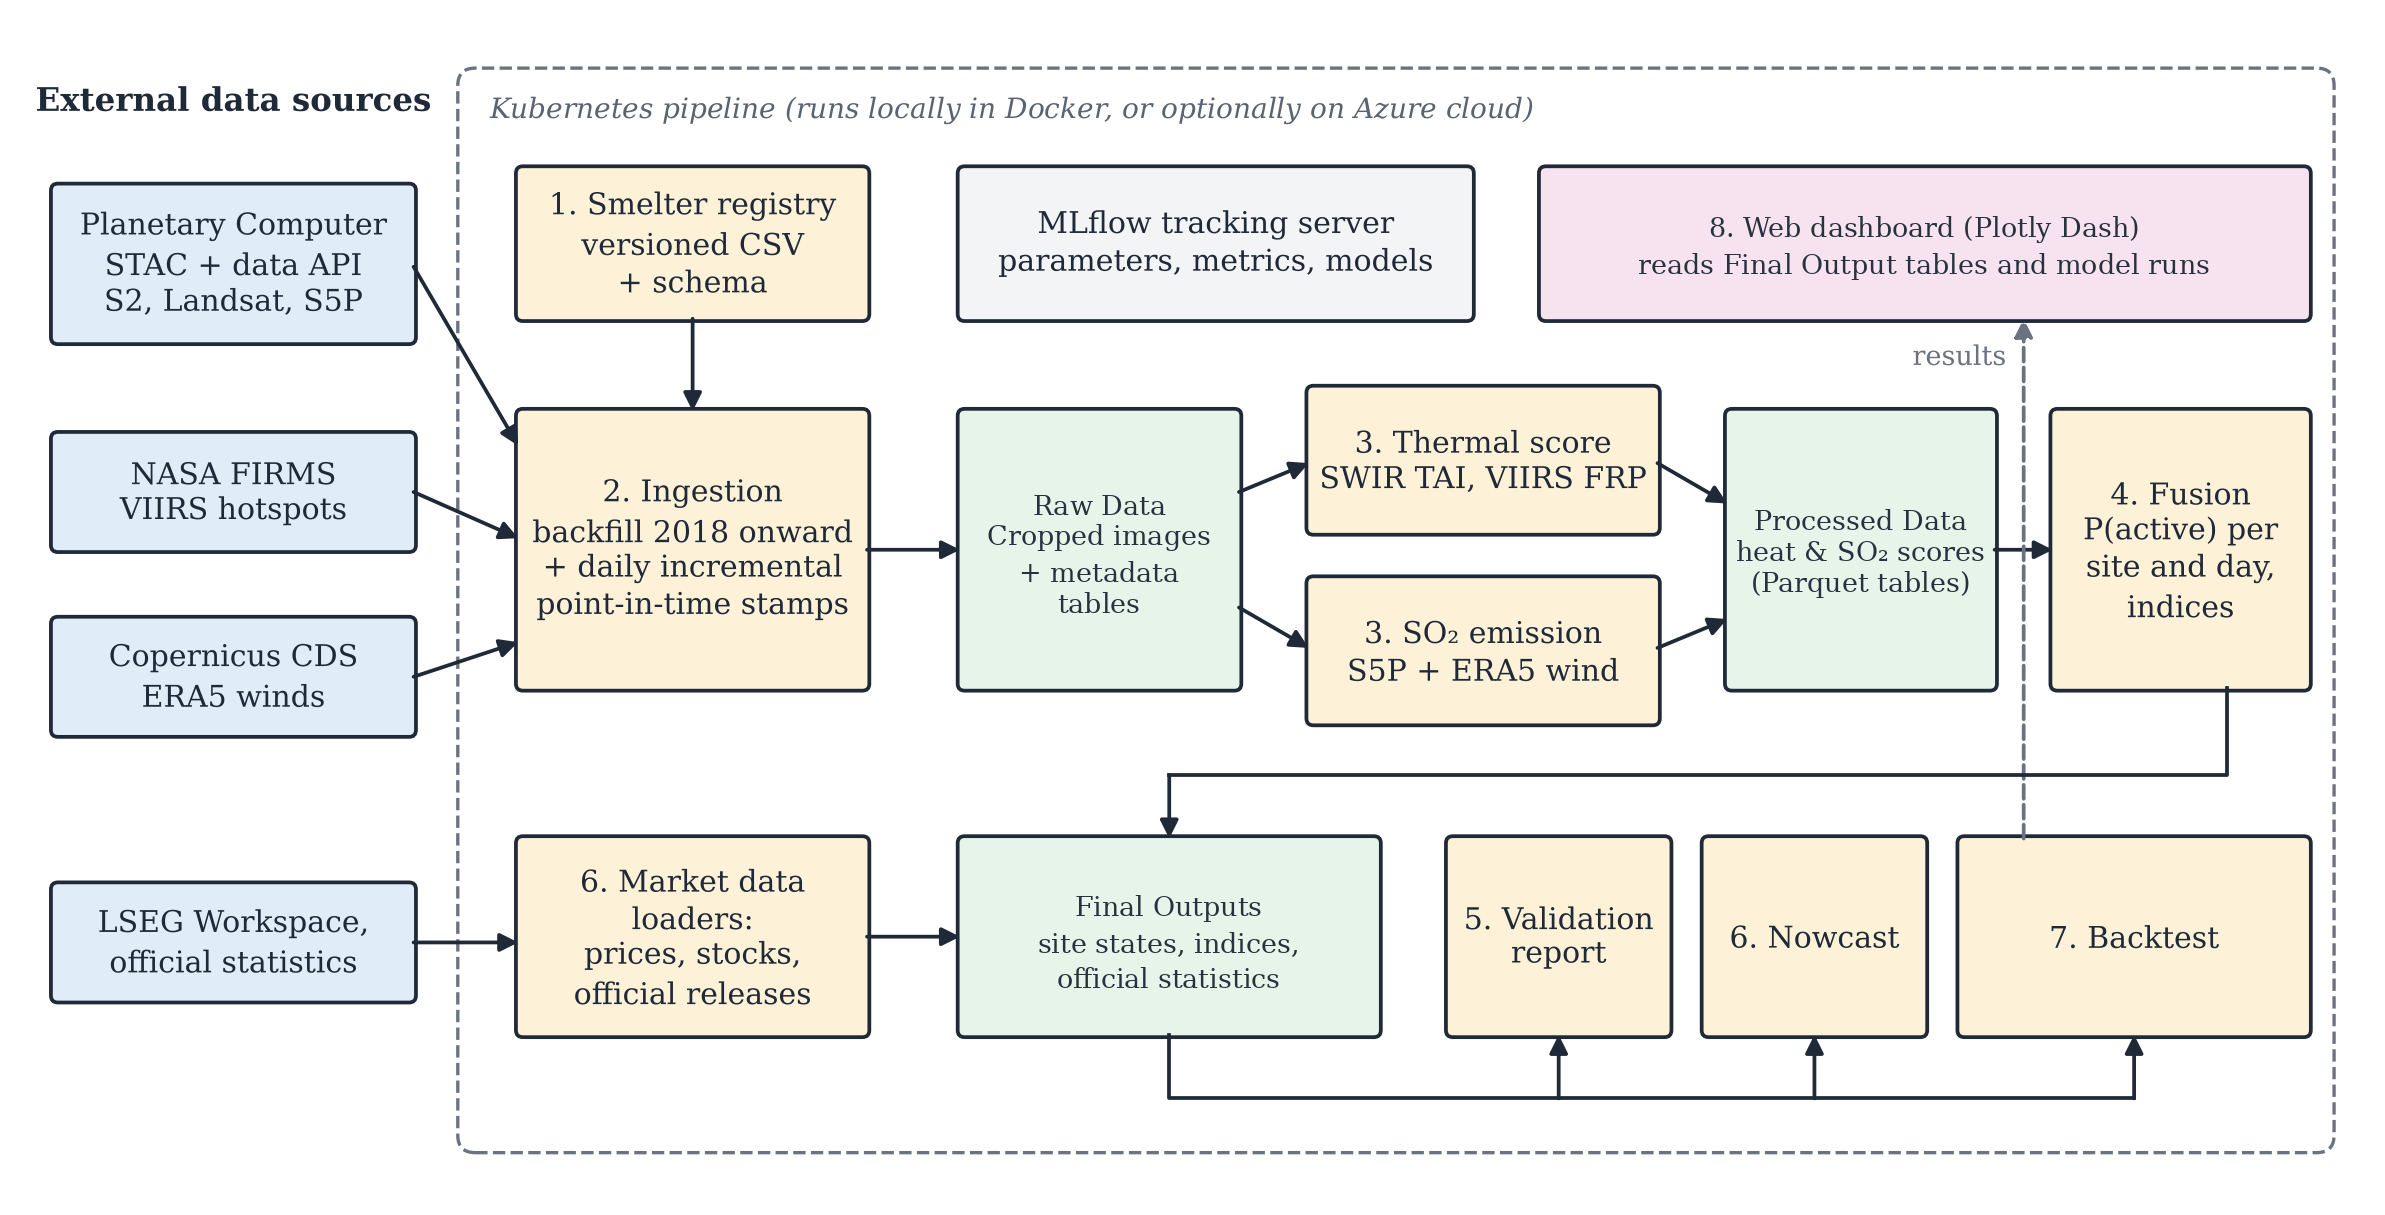
\includegraphics[width=6.6in,height=3.36226in]{figures/architecture.png}

Fig. 1. Planned system architecture. Numbers refer to the requirements
in Section II. Yellow boxes are processing scripts managed by
Kubernetes; green boxes are our three data storage stages (Raw Data,
Processed Data, and Final Outputs saved as Parquet/CSV tables). The
smelter registry (1) defines the coordinates used to download data, and
the Final Outputs feed validation, nowcasting, backtesting, and the web
dashboard.

\hypertarget{a.-requirement-1-smelter-registry}{%
\subsection{A. Requirement 1: Smelter
Registry}\label{a.-requirement-1-smelter-registry}}

We will create and maintain a CSV file (\emph{smelter\_registry.csv}) in
our GitHub repository containing the 30 largest copper smelters in the
world. A simple CSV file is easy for the whole team to edit and review.
Each row will store a unique smelter ID, plant name, operator, country,
region, annual production capacity, GPS coordinates (latitude and
longitude), and a link to the public source where we found the
information. Using the GPS coordinates, a helper script will define two
capture zones around each smelter: a small 1.5 km square to check for
furnace heat, and a 50 km circle to check for SO₂ gas plumes.

\begin{longtable}[]{@{}
  >{\raggedright\arraybackslash}p{(\columnwidth - 0\tabcolsep) * \real{1.0000}}@{}}
\toprule\noalign{}
\begin{minipage}[b]{\linewidth}\raggedright
\textbf{\emph{Algorithm 1. Checking and saving the smelter list}}

Function CheckSmelterRegistry(csv\_file):

\begin{quote}
table = read\_csv(csv\_file)

for each smelter in table:

if smelter.id is missing or duplicated:

stop\_with\_error(\textquotesingle Missing or duplicate
ID\textquotesingle)

if smelter.lat or smelter.lon is invalid:

stop\_with\_error(\textquotesingle Invalid GPS
coordinates\textquotesingle)

if smelter.capacity \textless= 0 or smelter.source\_url is empty:

stop\_with\_error(\textquotesingle Missing capacity or source
link\textquotesingle)

smelter.heat\_box = make\_square(smelter.lat, smelter.lon, 1.5 km)

smelter.gas\_circle = make\_circle(smelter.lat, smelter.lon, 50 km)

save\_table(table,
\textquotesingle clean\_smelter\_registry.csv\textquotesingle)
\end{quote}
\end{minipage} \\
\midrule\noalign{}
\endhead
\bottomrule\noalign{}
\endlastfoot
 \\
\end{longtable}

Whenever a team member updates the CSV file on GitHub, an automated test
will run this check to make sure no required fields or sources are
missing. \emph{Acceptance:} a verified table of 30 smelters with GPS
coordinates, capacities, and cited sources.

\hypertarget{b.-requirement-2-satellite-data-ingestion}{%
\subsection{B. Requirement 2: Satellite Data
Ingestion}\label{b.-requirement-2-satellite-data-ingestion}}

This module downloads historical satellite and weather data from 2018 to
the present for all 30 smelters, and then checks for new images once a
day. Full satellite images are very large, so we will use the Planetary
Computer API to download only the small cropped area around each smelter
for Sentinel-2 and Landsat (shortwave-infrared bands and cloud masks).
Night-time heat points will be downloaded from the NASA FIRMS API,
Sentinel-5P SO₂ data will be fetched for the 50 km circle, and ERA5 wind
data will be downloaded from the Copernicus API.

\begin{longtable}[]{@{}
  >{\raggedright\arraybackslash}p{(\columnwidth - 0\tabcolsep) * \real{1.0000}}@{}}
\toprule\noalign{}
\begin{minipage}[b]{\linewidth}\raggedright
\textbf{\emph{Algorithm 2. Downloading historical and daily satellite
data}}

Function DownloadSatelliteData(smelters, start\_date, end\_date):

\begin{quote}
for each smelter in smelters:

for each sensor in {[}Sentinel2, Landsat, VIIRS, Sentinel5P, ERA5{]}:

images = search\_api(sensor, smelter.zone, start\_date, end\_date)

for each img in images:

if already\_downloaded(raw\_data\_folder, img.id):

continue to next img

crop = download\_cropped\_area(img, smelter.zone)

obs\_date = img.capture\_time

avail\_date = obs\_date + sensor.typical\_delay

save\_to\_raw\_data(crop, smelter.id, sensor, obs\_date, avail\_date)
\end{quote}

Daily schedule (runs once per day):

\begin{quote}
DownloadSatelliteData(smelters, yesterday, today)
\end{quote}
\end{minipage} \\
\midrule\noalign{}
\endhead
\bottomrule\noalign{}
\endlastfoot
 \\
\end{longtable}

If a file is already in our \textbf{Raw Data} folder, the script skips
it so we can easily pause and resume downloads without starting over.
Because free APIs have rate limits (such as NASA FIRMS {[}15{]}), the
script will pause briefly between requests if needed. \emph{Acceptance:}
complete historical data from 2018 onward for all 30 smelters, plus a
daily update script.

\hypertarget{c.-requirement-3-site-activity-detection}{%
\subsection{C. Requirement 3: Site Activity
Detection}\label{c.-requirement-3-site-activity-detection}}

\emph{Thermal score.} Smelter furnaces are extremely hot and glow in
shortwave-infrared (SWIR) satellite bands. For each Sentinel-2 or
Landsat image in our \textbf{Raw Data} folder, we first check the cloud
mask band. If more than 30\% of the 1.5 km box is covered by clouds, we
mark the image as cloudy and skip it so we do not confuse clouds with an
inactive smelter. On clear images, we use a published SWIR band ratio
{[}6{]} to count how many abnormally hot pixels appear inside the box.
For VIIRS night-time data, we count the number of heat detections within
1.5 km of the smelter and add up their heat intensity (FRP) {[}14{]}.

\emph{SO₂ emission score.} When a smelter processes copper ore, it
releases sulfur dioxide (SO₂) gas. For each Sentinel-5P pass over a
smelter, we keep only good-quality pixels inside the 50 km circle and
combine them with ERA5 wind speed and direction to estimate the SO₂
emission level (using either a simple wind-aligned average or the
open-source \emph{ddeq} Python library {[}8{]}).

\begin{longtable}[]{@{}
  >{\raggedright\arraybackslash}p{(\columnwidth - 0\tabcolsep) * \real{1.0000}}@{}}
\toprule\noalign{}
\begin{minipage}[b]{\linewidth}\raggedright
\textbf{\emph{Algorithm 3. Computing heat and gas scores for each
observation}}

For each new\_file in raw\_data\_folder:

\begin{quote}
if new\_file.sensor in {[}Sentinel2, Landsat{]}:

clouds = get\_cloud\_percentage(new\_file.quality\_band)

if clouds \textgreater{} 30\%:

quality = \textquotesingle CLOUDY\textquotesingle; score = None

else:

hot\_pixels = count\_pixels(SWIR\_formula \textgreater{}
heat\_threshold)

quality = \textquotesingle GOOD\textquotesingle; score = hot\_pixels

else if new\_file.sensor == VIIRS:

points = get\_night\_hotspots\_within\_1\_5km(new\_file)

quality = \textquotesingle GOOD\textquotesingle; score =
sum(points.heat\_power)

else if new\_file.sensor == Sentinel5P:

pixels = keep\_good\_pixels(new\_file, qa\_value \textgreater= 0.5)

wind = get\_era5\_wind(new\_file.smelter, new\_file.obs\_date)

score = estimate\_so2\_emission(pixels, wind)

quality = \textquotesingle GOOD\textquotesingle{} if pixels\_sufficient
else \textquotesingle LOW\_QUALITY\textquotesingle{}

save\_to\_processed\_data(new\_file.smelter, new\_file.sensor, score,
quality)
\end{quote}
\end{minipage} \\
\midrule\noalign{}
\endhead
\bottomrule\noalign{}
\endlastfoot
 \\
\end{longtable}

\emph{Acceptance:} a clean \textbf{Processed Data} table containing a
heat or gas score and a quality flag for every satellite observation.

\hypertarget{d.-requirement-4-fusion-and-activity-indices}{%
\subsection{D. Requirement 4: Fusion and Activity
Indices}\label{d.-requirement-4-fusion-and-activity-indices}}

A single satellite pass is often incomplete because of clouds or wind,
so we combine all sensors to estimate a daily probability
(\emph{P\_active} between 0 and 1) that each smelter is operating. We
model each smelter as having two possible daily states, \emph{ON} or
\emph{OFF}, using a basic Hidden Markov Model (Fig. 2) {[}17{]}. Because
smelters normally run for months at a time, we start each day with
yesterday\textquotesingle s probability. When clear heat or gas scores
are available in our \textbf{Processed Data} table for that day, the
model increases \emph{P\_active} if heat or gas was seen, or decreases
it if the sky was clear but no activity was detected. On cloudy days
with no usable data, the probability simply stays close to
yesterday\textquotesingle s value instead of dropping to zero.

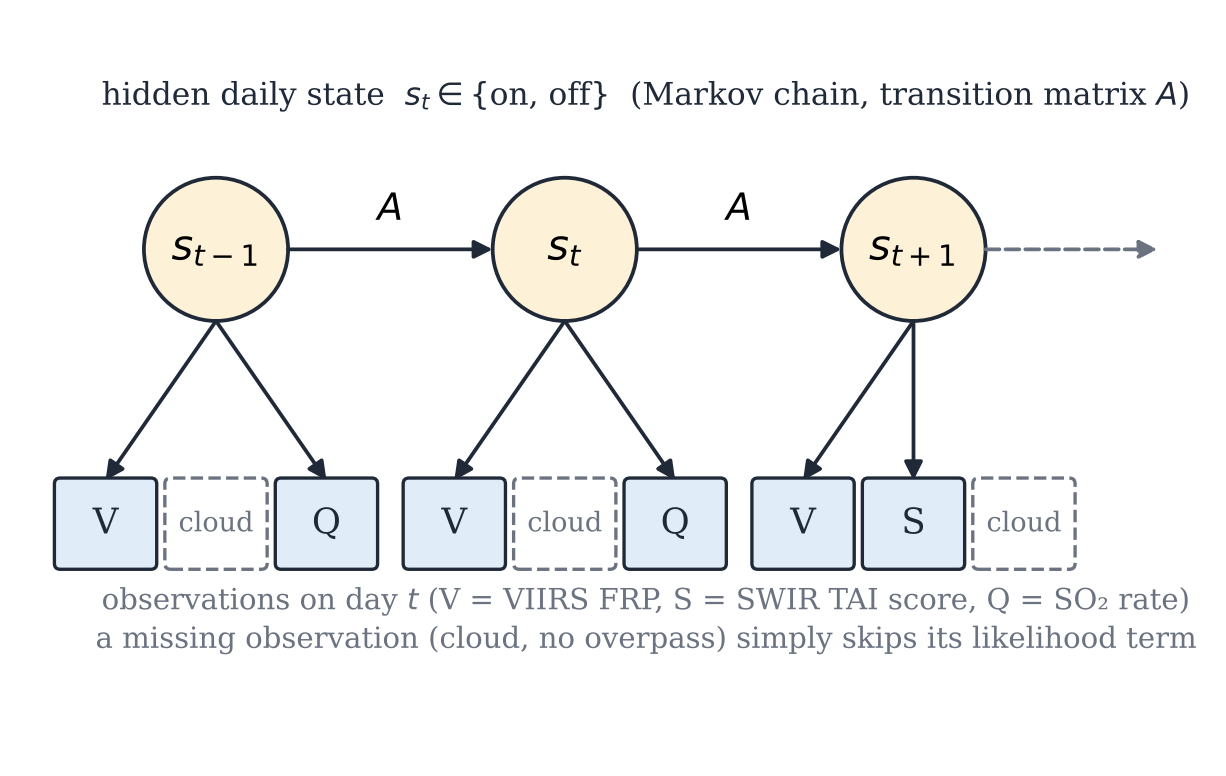
\includegraphics[width=3.2in,height=2.02545in]{figures/fusion.png}

Fig. 2. Fusion model for one site. The daily on/off state is hidden;
each sensor gives an observation only when it passes over in clear sky.

\begin{longtable}[]{@{}
  >{\raggedright\arraybackslash}p{(\columnwidth - 0\tabcolsep) * \real{1.0000}}@{}}
\toprule\noalign{}
\begin{minipage}[b]{\linewidth}\raggedright
\textbf{\emph{Algorithm 4. Daily sensor fusion and regional index
calculation}}

For each day t, for each smelter i:

\begin{quote}
prob\_active = yesterday\_probability(i, t - 1)

obs\_list = get\_processed\_data(i, day = t, available\_date \textless=
t)

for each obs in obs\_list:

if obs.quality == \textquotesingle GOOD\textquotesingle:

if obs.score \textgreater{} active\_threshold(obs.sensor):

prob\_active = update\_upward(prob\_active, obs.score)

else:

prob\_active = update\_downward(prob\_active, obs.score)

save\_to\_final\_outputs(\textquotesingle site\_state\textquotesingle,
i, t, prob\_active)
\end{quote}

For each region R in {[}World, China, Asia\_ex\_China, Americas, Europe,
Africa{]}:

\begin{quote}
weighted\_active = sum(smelter.capacity * prob\_active{[}smelter, t{]}
for smelter in R)

total\_capacity = sum(smelter.capacity for smelter in R)

Index{[}R, t{]} = 100 * (weighted\_active / total\_capacity)

save\_to\_final\_outputs(\textquotesingle indices\textquotesingle, R, t,
Index{[}R, t{]})
\end{quote}
\end{minipage} \\
\midrule\noalign{}
\endhead
\bottomrule\noalign{}
\endlastfoot
 \\
\end{longtable}

To avoid using future data, each day\textquotesingle s probability is
calculated using only observations already available on or before that
day. We then compute regional and global activity indices (from 0 to
100) by taking a weighted average of \emph{P\_active} using each
smelter\textquotesingle s production capacity from the registry, so
larger smelters have a bigger weight. \emph{Acceptance:} continuous
daily smelter probabilities and regional indices saved in our
\textbf{Final Outputs} folder from 2018 to the present.

\hypertarget{e.-requirement-5-validation}{%
\subsection{E. Requirement 5:
Validation}\label{e.-requirement-5-validation}}

Before using our indices for financial analysis, we will check whether
they match reality using three simple tests. First, we will create a
\textbf{known-events list} in CSV format containing 10 to 20 real
smelter shutdowns or maintenance stops reported in news articles, and
check whether our smelter probability drops below 0.5 during those
dates. Second, we will compare the monthly average of our regional
indices with official monthly copper production statistics (such as
Chinese and global production data). Third, we will compare our global
inactive percentage (\emph{100 - World\_Index}) with the headline
numbers occasionally shared in the press by SAVANT {[}4{]}.

\begin{longtable}[]{@{}
  >{\raggedright\arraybackslash}p{(\columnwidth - 0\tabcolsep) * \real{1.0000}}@{}}
\toprule\noalign{}
\begin{minipage}[b]{\linewidth}\raggedright
\textbf{\emph{Algorithm 5. Checking accuracy against real events and
official data}}

events =
read\_csv(\textquotesingle known\_shutdown\_events.csv\textquotesingle)

detected\_count = 0

for each event in events:

\begin{quote}
probs =
get\_final\_outputs(\textquotesingle site\_state\textquotesingle,
event.smelter, event.start, event.end)

if average(probs) \textless{} 0.5:

detected\_count = detected\_count + 1
\end{quote}

detection\_rate = detected\_count / total\_events

for each region in {[}World, China{]}:

\begin{quote}
monthly\_index = compute\_monthly\_average(Index{[}region{]})

corr\_score = correlation(monthly\_index,
official\_monthly\_output{[}region{]})
\end{quote}

save\_validation\_report(detection\_rate, corr\_score)
\end{minipage} \\
\midrule\noalign{}
\endhead
\bottomrule\noalign{}
\endlastfoot
 \\
\end{longtable}

\emph{Acceptance:} a summary validation report showing the shutdown
detection rate and correlation with official monthly copper output.

\hypertarget{f.-requirement-6-market-data-and-nowcasting}{%
\subsection{F. Requirement 6: Market Data and
Nowcasting}\label{f.-requirement-6-market-data-and-nowcasting}}

We will collect copper futures prices (COMEX, LME, SHFE), exchange
inventory levels, and official monthly copper production figures from
\textbf{LSEG Workspace} (which one team member has access to) and public
statistical releases. Because the LSEG account is for individual student
use, raw LSEG files will stay on that teammate\textquotesingle s
computer and only summary charts and test results will be shown in the
dashboard. For official monthly production numbers, we also record the
exact publication date (\emph{available\_date}) so our tests know when
each report became public.

Official production statistics come out weeks after the end of the
month. To estimate the current month\textquotesingle s production early
(nowcasting), we will use a simple linear regression model (such as
Ridge regression in \emph{scikit-learn}) that predicts monthly
production from our month-to-date satellite index average and the last
published official number {[}18{]}. We will compare its error against a
simple baseline that just guesses the previous month\textquotesingle s
value.

\begin{longtable}[]{@{}
  >{\raggedright\arraybackslash}p{(\columnwidth - 0\tabcolsep) * \real{1.0000}}@{}}
\toprule\noalign{}
\begin{minipage}[b]{\linewidth}\raggedright
\textbf{\emph{Algorithm 6. Predicting monthly copper production
(Nowcasting)}}

For each day d inside month m:

\begin{quote}
\# Use only past months whose official report was already published
before day d

past\_months = get\_months\_published\_before(d)

X\_train = {[}mean\_index\_in\_month(k) for k in past\_months{]}

y\_train = {[}official\_production(k) for k in past\_months{]}

model = LinearRegression().fit(X\_train, y\_train)

X\_current = mean\_index\_so\_far(month = m, up\_to\_day = d)

prediction = model.predict(X\_current)

save\_to\_final\_outputs(\textquotesingle nowcast\textquotesingle, month
= m, day = d, value = prediction)
\end{quote}
\end{minipage} \\
\midrule\noalign{}
\endhead
\bottomrule\noalign{}
\endlastfoot
 \\
\end{longtable}

\emph{Acceptance:} monthly production estimates that achieve a lower
prediction error than the simple baseline guess.

\hypertarget{g.-requirement-7-backtesting}{%
\subsection{G. Requirement 7:
Backtesting}\label{g.-requirement-7-backtesting}}

We will test a simple trading strategy on COMEX copper futures {[}21{]}
driven by changes in our global smelter activity index. The intuition is
straightforward: if the global smelter activity index drops noticeably
over the last 20 days, it suggests smelters are shutting down and
refined copper supply may tighten, so the strategy buys copper futures
(goes long). If smelter activity rises strongly, the strategy sells or
reduces its position. On each simulated day, the script only reads rows
from \textbf{Final Outputs} whose \emph{available\_date} is on or before
that day, preventing any look-ahead bias.

\begin{longtable}[]{@{}
  >{\raggedright\arraybackslash}p{(\columnwidth - 0\tabcolsep) * \real{1.0000}}@{}}
\toprule\noalign{}
\begin{minipage}[b]{\linewidth}\raggedright
\textbf{\emph{Algorithm 7. Simulating the copper futures trading
strategy}}

position = 0; total\_pnl = 0

For each trading\_day t in backtest\_period:

\begin{quote}
\# Only read index values that were available on or before day t

index\_history =
get\_final\_outputs(\textquotesingle indices\textquotesingle,
\textquotesingle World\textquotesingle, available\_date \textless= t)

index\_change = index\_history{[}t{]} - index\_history{[}t - 20 days{]}

if index\_change \textless{} -buy\_threshold:

target\_pos = +1 \# Buy futures (smelter activity dropped
-\textgreater{} tighter supply)

else if index\_change \textgreater{} +sell\_threshold:

target\_pos = -1 \# Sell futures (smelter activity rose -\textgreater{}
higher supply)

else:

target\_pos = 0

trade\_cost = abs(target\_pos - position) * fee\_per\_trade

daily\_pnl = position * (price{[}t{]} - price{[}t - 1{]}) - trade\_cost

position = target\_pos

save\_daily\_pnl(t, daily\_pnl)
\end{quote}

Compute summary metrics: annual return, volatility, Sharpe ratio, max
drawdown
\end{minipage} \\
\midrule\noalign{}
\endhead
\bottomrule\noalign{}
\endlastfoot
 \\
\end{longtable}

We subtract a fixed transaction fee and price slippage whenever the
position changes, and compare the strategy\textquotesingle s return,
maximum drawdown, and Sharpe ratio {[}19{]} against a basic buy-and-hold
benchmark. \emph{Acceptance:} a reproducible backtest simulation saved
to \textbf{Final Outputs} and MLflow so its profit curve and metrics can
be viewed in the dashboard.

\hypertarget{h.-requirement-8-dashboard}{%
\subsection{H. Requirement 8:
Dashboard}\label{h.-requirement-8-dashboard}}

The dashboard is a Plotly Dash web application running in a container so
anyone on the team can open it in a browser. It uses DuckDB to read our
\textbf{Final Outputs} tables directly and displays five simple tabs: a
\textbf{world map} of the 30 smelters colored by their current
\emph{P\_active} status; a \textbf{smelter detail page} showing a
smelter\textquotesingle s heat and SO₂ history along with cropped
satellite images; the \textbf{regional activity indices}; the
\textbf{monthly production nowcasts} compared with official releases;
and the \textbf{backtest results}. A date selector lets the user pick
any past date and view the dashboard using only data that was available
on that day.

\begin{longtable}[]{@{}
  >{\raggedright\arraybackslash}p{(\columnwidth - 0\tabcolsep) * \real{1.0000}}@{}}
\toprule\noalign{}
\begin{minipage}[b]{\linewidth}\raggedright
\textbf{\emph{Algorithm 8. Updating the web dashboard when a user picks
a date}}

app = Dash()

When user selects (selected\_date, selected\_region) on the webpage:

\begin{quote}
sites\_df = duckdb.query(

\textquotesingle SELECT * FROM final\_outputs.site\_state WHERE
available\_date \textless= ?\textquotesingle, {[}selected\_date{]}

)

index\_df = duckdb.query(

\textquotesingle SELECT * FROM final\_outputs.indices WHERE region = ?
AND available\_date \textless= ?\textquotesingle,

{[}selected\_region, selected\_date{]}

)

return draw\_map(sites\_df), draw\_line\_chart(index\_df)
\end{quote}
\end{minipage} \\
\midrule\noalign{}
\endhead
\bottomrule\noalign{}
\endlastfoot
 \\
\end{longtable}

\emph{Acceptance:} all dashboard tabs load in under 3 seconds on our
laptops, and clicking a smelter shows the underlying satellite
observations.

\hypertarget{references-part-i}{%
\section{References (Part I)}\label{references-part-i}}

{[}1{]} Earth-i, ``Metals Smelting Insight.'' {[}Online{]}. Available:
https://earthi.space/services/savant-metals-smelting-insight/ (accessed
Oct.~22, 2026).

{[}2{]} Earth-i, ``Earth-i announces launch of the SAVANT Global Copper
Smelting Index,'' Oct.~8, 2019. {[}Online{]}. Available:
https://earthi.space/?p=5293

{[}3{]} MINING.COM, ``Satellites to monitor copper supply from space,''
Oct. 9, 2019. {[}Online{]}. Available:
https://www.mining.com/satellites-to-monitor-copper-supply-from-space/

{[}4{]} Shanghai Metals Market, ``Satellite-based monitoring firm state
primary smelter activity remains strong,'' Nov.~18, 2025. {[}Online{]}.
Available:
https://news.metal.com/newscontent/103625040-satellite-based-monitoring-firm-state-primary-smelter-activity-remains-strong

{[}5{]} Climate TRACE, ``Conversations with the Coalition:
TransitionZero,'' Jul.~23, 2024. {[}Online{]}. Available:
https://climatetrace.org/news/conversations-with-the-coalition-transitionzero

{[}6{]} F. Massimetti, D. Coppola, M. Laiolo, S. Valade, C. Cigolini,
and M. Ripepe, ``Volcanic hot-spot detection using SENTINEL-2: A
comparison with MODIS--MIROVA thermal data series,'' Remote Sens.,
vol.~12, no. 5, Art. no. 820, 2020, doi: 10.3390/rs12050820.

{[}7{]} V. E. Fioletov et al., ``A global catalogue of large SO₂ sources
and emissions derived from the Ozone Monitoring Instrument,'' Atmos.
Chem. Phys., vol.~16, pp.~11497--11519, 2016, doi:
10.5194/acp-16-11497-2016.

{[}8{]} G. Kuhlmann et al., ``The ddeq Python library for point source
quantification from remote sensing images (version 1.0),'' Geosci. Model
Dev., vol.~17, pp.~4773--4789, 2024, doi: 10.5194/gmd-17-4773-2024.

{[}9{]} D. P. Finch and P. I. Palmer, ``Towards automated near-real-time
global monitoring of atmospheric SO₂ plumes from satellite data using
U-Net segmentation,'' Atmos. Meas. Tech., vol.~19, pp.~4049--4064, 2026,
doi: 10.5194/amt-19-4049-2026.

{[}10{]} Microsoft, ``Planetary Computer data catalog.'' {[}Online{]}.
Available: https://planetarycomputer.microsoft.com/catalog (accessed
Oct.~22, 2026).

{[}11{]} Microsoft, ``Azure for Students.'' {[}Online{]}. Available:
https://azure.microsoft.com/free/students/

{[}12{]} Microsoft, ``Azure Kubernetes Service (AKS) pricing.''
{[}Online{]}. Available:
https://azure.microsoft.com/pricing/details/kubernetes-service/

{[}13{]} Argo Project, ``Argo Workflows documentation.'' {[}Online{]}.
Available: https://argo-workflows.readthedocs.io/

{[}14{]} W. Schroeder, P. Oliva, L. Giglio, and I. A. Csiszar, ``The New
VIIRS 375 m active fire detection data product: Algorithm description
and initial assessment,'' Remote Sens. Environ., vol.~143, pp.~85--96,
2014, doi: 10.1016/j.rse.2013.12.008.

{[}15{]} NASA LANCE, ``FIRMS API.'' {[}Online{]}. Available:
https://firms.modaps.eosdis.nasa.gov/api/ (accessed Nov.~4, 2026).

{[}16{]} N. Theys et al., ``Sulfur dioxide retrievals from TROPOMI
onboard Sentinel-5 Precursor: algorithm theoretical basis,'' Atmos.
Meas. Tech., vol.~10, pp.~119--153, 2017, doi: 10.5194/amt-10-119-2017.

{[}17{]} L. R. Rabiner, ``A tutorial on hidden Markov models and
selected applications in speech recognition,'' Proc. IEEE, vol.~77, no.
2, pp. 257--286, 1989, doi: 10.1109/5.18626.

{[}18{]} D. Giannone, L. Reichlin, and D. Small, ``Nowcasting: The
real-time informational content of macroeconomic data,'' J. Monetary
Econ., vol.~55, no. 4, pp.~665--676, 2008, doi:
10.1016/j.jmoneco.2008.05.010.

{[}19{]} D. H. Bailey and M. López de Prado, ``The deflated Sharpe
ratio: Correcting for selection bias, backtest overfitting, and
non-normality,'' J. Portfolio Manage., vol.~40, no. 5, pp.~94--107,
2014, doi: 10.3905/jpm.2014.40.5.094.

{[}20{]} H. Hersbach et al., ``The ERA5 global reanalysis,'' Q. J. R.
Meteorol. Soc., vol.~146, pp.~1999--2049, 2020, doi: 10.1002/qj.3803.

{[}21{]} CME Group, ``Copper futures contract specs.'' {[}Online{]}.
Available:
https://www.cmegroup.com/markets/metals/base/copper.contractSpecs.html

\part{Technical Report: Work Done So Far}

This part documents the work carried out since the proposal (status of
November 2026): the smelter registry, the data sources, the ingestion
code, the first prototype and the difficulties met.

\hypertarget{background-where-to-observe-copper}{%
\section{1. Background: Where to Observe
Copper}\label{background-where-to-observe-copper}}

OrbitCu observes the smelter (smelting, converting and fire refining in
the figure below), because it is the only stage of the copper chain with
a signature visible from space. Smelting and converting run at furnace
temperatures and burn the sulfur in the concentrate, which produces both
intense shortwave-infrared heat and SO₂.

\textbf{Copper life cycle in brief.} Sulfide ore (0.5--1\% Cu) is mined
and concentrated by flotation to 25--35\% Cu. The smelter melts the
concentrate into matte (50--70\% Cu), converts it to blister (98--99\%)
and fire-refines it into anodes (99.5\%). Electrorefining then produces
cathode (99.99\%), the traded commodity, which is semi-fabricated into
rod and wire, built into products and, at end of life, partly returned
as scrap to smelters and refineries.

\begin{figure}
\centering
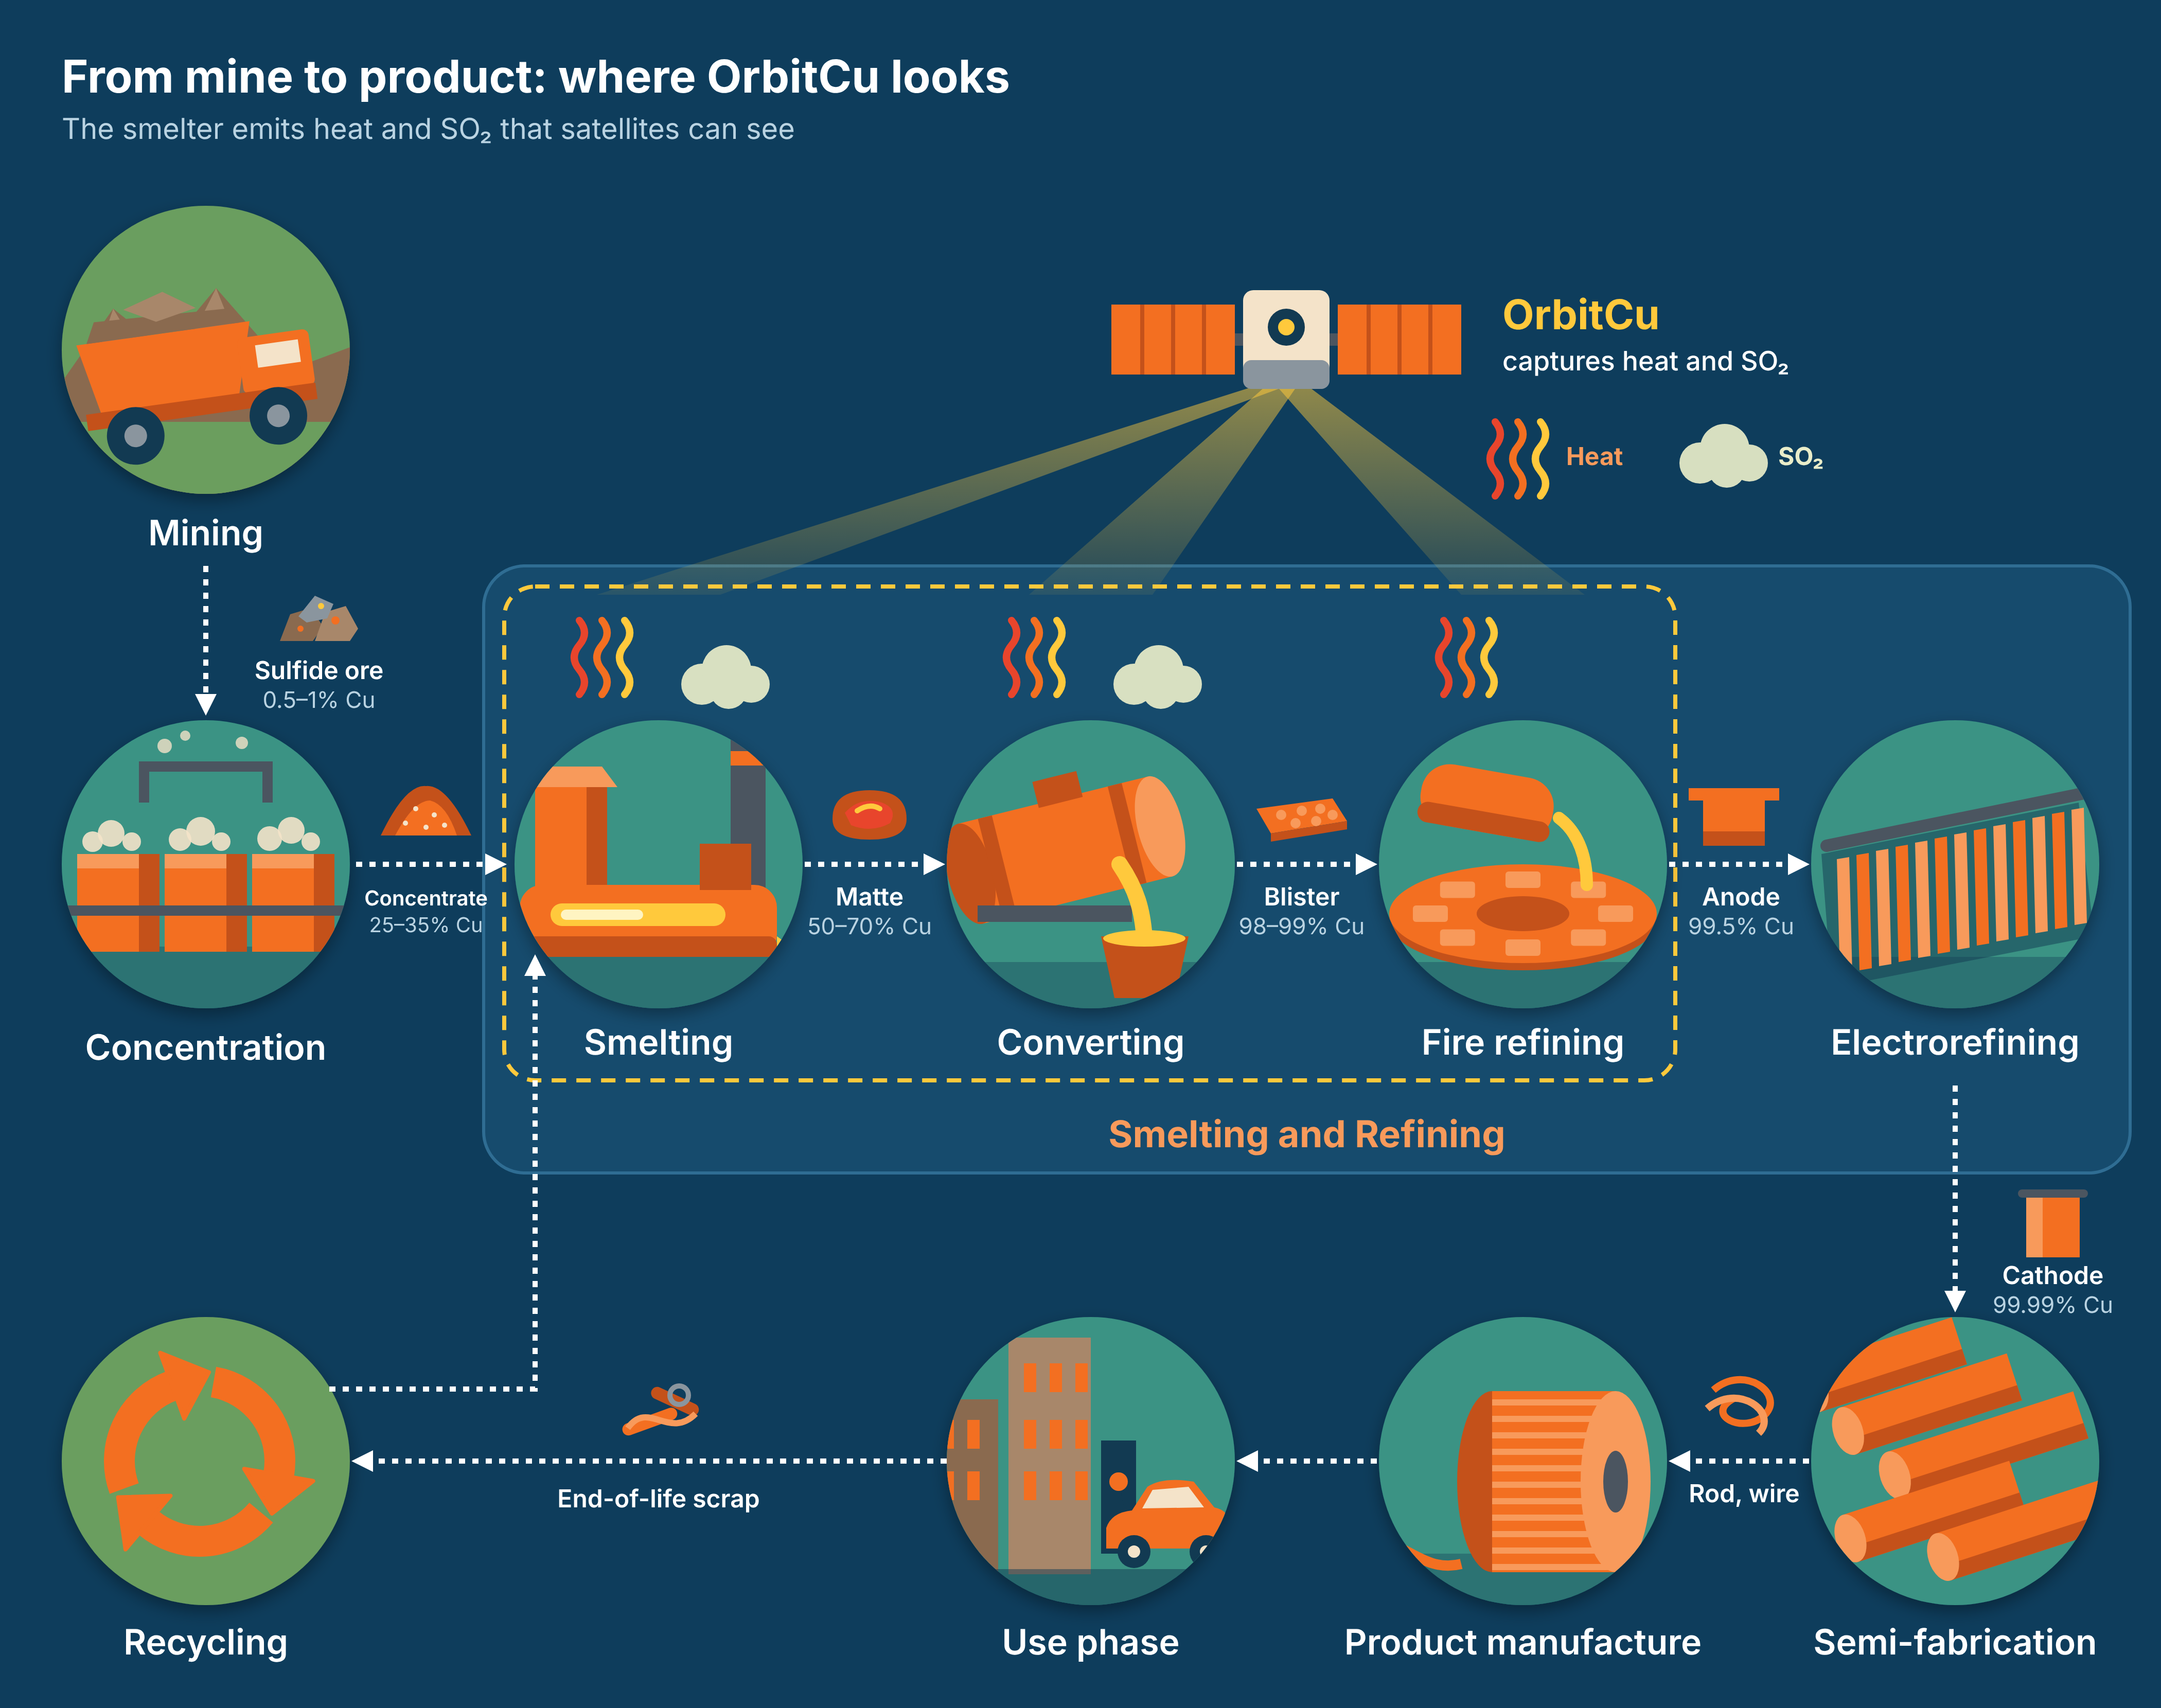
\includegraphics[width=0.95\textwidth,height=\textheight]{figures/copper_value_chain.png}
\caption{Copper value chain from mine to product, with the smelting
stages observed by OrbitCu}
\end{figure}

The other stages are not observable or are out of scope. Mines and
concentrators are out of scope. Electrorefineries use low-temperature
electrolysis and emit neither heat nor SO₂. Refined supply that bypasses
smelters (SX-EW cathode from leached oxide ores, and scrap) is invisible
to OrbitCu, which limits how much of refined output the indices can
explain. For the same reason, registry capacities should be expressed as
blister or anode copper, the output of the observed stages.

\hypertarget{satellite-data-sources-and-access-platforms}{%
\section{2. Satellite Data Sources and Access
Platforms}\label{satellite-data-sources-and-access-platforms}}

OrbitCu uses five free datasets reached through three access platforms.
Sources are grouped by platform because access keys, quotas and failure
modes are set per platform, not per satellite.

\begin{longtable}[]{@{}
  >{\raggedright\arraybackslash}p{(\columnwidth - 8\tabcolsep) * \real{0.2000}}
  >{\raggedright\arraybackslash}p{(\columnwidth - 8\tabcolsep) * \real{0.2000}}
  >{\raggedright\arraybackslash}p{(\columnwidth - 8\tabcolsep) * \real{0.2000}}
  >{\raggedright\arraybackslash}p{(\columnwidth - 8\tabcolsep) * \real{0.2000}}
  >{\raggedright\arraybackslash}p{(\columnwidth - 8\tabcolsep) * \real{0.2000}}@{}}
\toprule\noalign{}
\begin{minipage}[b]{\linewidth}\raggedright
Platform
\end{minipage} & \begin{minipage}[b]{\linewidth}\raggedright
Datasets (sensor)
\end{minipage} & \begin{minipage}[b]{\linewidth}\raggedright
Signal for OrbitCu
\end{minipage} & \begin{minipage}[b]{\linewidth}\raggedright
Resolution and timeliness
\end{minipage} & \begin{minipage}[b]{\linewidth}\raggedright
Main limits
\end{minipage} \\
\midrule\noalign{}
\endhead
\bottomrule\noalign{}
\endlastfoot
Microsoft Planetary Computer, STAC API {[}10{]}, {[}16{]} & Sentinel-2
L2A (MSI); Landsat Collection 2 L2 (OLI/TIRS); Sentinel-5P L2 (TROPOMI)
& Furnace heat in SWIR (S2 B11 1.61 µm, B12 2.19 µm; Landsat SWIR
1.6/2.2 µm); SO₂ total column (S5P) & S2: 20 m SWIR, about 5-day
revisit, archive since 2015. Landsat: 30 m SWIR, 100 m surface
temperature. S5P: 5.5 × 3.5 km pixels, daily, since April 2018 & Daytime
optical passes masked by cloud; files sit on Azure Blob Storage behind
short-lived SAS tokens (about 1 h); SO₂ from smaller smelters close to
the detection limit \\
NASA FIRMS (LANCE) {[}17{]} & VIIRS 375 m active fire (S-NPP, NOAA-20,
NOAA-21); MODIS & Night-time thermal anomalies at each site & Global
near-real-time detections within 3 hours of overpass; separate
standard-processing archive & Free MAP\_KEY limited to 5,000
transactions per 10 minutes; at most 5 days per area request; product
tuned for fires, 375 m footprint, no detection under cloud \\
Copernicus Climate Data Store (C3S, ECMWF) {[}18{]} & ERA5 hourly
reanalysis on single levels & Wind fields that turn SO₂ columns into
emission rates & 0.25° grid, hourly, since 1940; daily update with about
5 days latency (ERA5T), final release 2--3 months later & Licence must
be accepted per account; requests are queued; ERA5T values can be
revised, so the availability date must be stored for point-in-time
use \\
\end{longtable}

\textbf{Access status (4 November 2026).} From the project's cloud
environment, the Planetary Computer STAC catalogue and its pixel cut-out
API (Sentinel-2, Landsat), the FIRMS key and the CDS key all work. Two
downloads remain blocked by the network allow-list: Sentinel-5P files,
which the catalogue serves from sentinel5euwest.blob.core.windows.net,
and CDS result files, served from an ECMWF object store. The ERA5
licence was accepted on 4 November and a test request is queued.
Backfill covers 2018 to present, then incremental ingestion as new
acquisitions are published.

\hypertarget{smelter-registry}{%
\section{3. Smelter Registry}\label{smelter-registry}}

The draft registry lists 29 primary copper smelters with about 11.7
Mt/yr of combined capacity (28 sites with a copper figure); slot 30 is
deliberately left open. Each site was checked against documents
published by its operator (annual and interim reports, securities
filings, results presentations, company web pages). 8 sites have both a
dated 2025-2026 operator confirmation of activity and an operator
capacity figure (A), 11 have a dated operator confirmation of activity
but no site capacity from the operator (B), and 10 have no dated
operator confirmation (C). The quotes, dates and links for each site are
in smelter\_registry\_draft.csv.

\textbf{Selection rules.} Only smelters are included, because refineries
(electrolysis) emit neither furnace heat nor SO₂. A site is kept if no
source reports it closed or suspended as of November 2026; sites
restarting in 2026 are kept with a flag. Sites are ranked by nameplate
capacity in kt of copper per year.

\textbf{Caveat on capacity.} No free, current, plant-level capacity
table exists: the ICSG directory, Statista and Wood Mackenzie are
paywalled. Figures therefore mix years (2015 to 2026) and stages
(blister, anode or cathode), and sources can disagree widely (Onahama:
354 kt in 2020 vs 230 kt in 2026). Capacities must be harmonised to
blister or anode copper before computing indices.

\textbf{Operator check levels.} \emph{A}: a dated 2025-2026 operator
document confirms that the site is operating, restarting or temporarily
halted, and the operator publishes a capacity figure for the site.
\emph{B}: a dated 2025-2026 operator document confirms activity, by
naming the site or reporting its output, but the capacity comes from a
secondary source. \emph{C}: no dated 2025-2026 operator document
confirming activity was found, because the operator does not publish
site data, its website refuses automated access (Xiangguang, Dongying
Fangyuan, Daye, NICICO), or the document could not be read. C sites need
satellite confirmation first.

\begin{longtable}[]{@{}
  >{\raggedright\arraybackslash}p{(\columnwidth - 10\tabcolsep) * \real{0.1667}}
  >{\raggedright\arraybackslash}p{(\columnwidth - 10\tabcolsep) * \real{0.1667}}
  >{\raggedright\arraybackslash}p{(\columnwidth - 10\tabcolsep) * \real{0.1667}}
  >{\raggedright\arraybackslash}p{(\columnwidth - 10\tabcolsep) * \real{0.1667}}
  >{\raggedright\arraybackslash}p{(\columnwidth - 10\tabcolsep) * \real{0.1667}}
  >{\raggedright\arraybackslash}p{(\columnwidth - 10\tabcolsep) * \real{0.1667}}@{}}
\caption{Registry of the 29 smelters (operator evidence grade A/B/C).
Quotes, dates and links for every site are in
\texttt{data/registry/smelter\_registry.csv}.}\tabularnewline
\toprule\noalign{}
\begin{minipage}[b]{\linewidth}\raggedright
\#
\end{minipage} & \begin{minipage}[b]{\linewidth}\raggedright
Smelter
\end{minipage} & \begin{minipage}[b]{\linewidth}\raggedright
Country
\end{minipage} & \begin{minipage}[b]{\linewidth}\raggedright
Operator
\end{minipage} & \begin{minipage}[b]{\linewidth}\raggedright
Capacity (kt Cu/yr)
\end{minipage} & \begin{minipage}[b]{\linewidth}\raggedright
Grade
\end{minipage} \\
\midrule\noalign{}
\endfirsthead
\toprule\noalign{}
\begin{minipage}[b]{\linewidth}\raggedright
\#
\end{minipage} & \begin{minipage}[b]{\linewidth}\raggedright
Smelter
\end{minipage} & \begin{minipage}[b]{\linewidth}\raggedright
Country
\end{minipage} & \begin{minipage}[b]{\linewidth}\raggedright
Operator
\end{minipage} & \begin{minipage}[b]{\linewidth}\raggedright
Capacity (kt Cu/yr)
\end{minipage} & \begin{minipage}[b]{\linewidth}\raggedright
Grade
\end{minipage} \\
\midrule\noalign{}
\endhead
\bottomrule\noalign{}
\endlastfoot
1 & Guixi & China & Jiangxi Copper & 900 & B \\
2 & Onsan & South Korea & LS MnM & 650 & C \\
3 & Kamoa-Kakula & DR Congo & Ivanhoe Mines / Zijin & 500 & A \\
4 & Kutch Copper (Mundra) & India & Adani Enterprises & 500 & A \\
5 & Birla Copper (Dahej) & India & Hindalco & 421 & A \\
6 & Jinguan (Tongling) & China & Tongling Nonferrous & 480 & B \\
7 & Glogow I + II & Poland & KGHM & 475 & A \\
8 & Chuquicamata & Chile & Codelco & 450 & C \\
9 & Jinchuan Fangchenggang & China & Jinchuan Group & 450 & C \\
10 & Hamburg & Germany & Aurubis & 450 & A \\
11 & Toyo (Niihama) & Japan & Sumitomo Metal Mining & 450 & C \\
12 & Saganoseki & Japan & JX Advanced Metals & 450 & B \\
13 & Chifeng Yunjin & China & Yunnan Copper (45\%) & 400 & B \\
14 & Southeast Copper (Ningde) & China & Yunnan Copper (60\%) / Chinalco
& 400 & B \\
15 & Xiangguang (Yanggu) & China & Xiangguang Copper (private) & 400 &
C \\
16 & Dongying Fangyuan & China & Dongying Fangyuan (private) & 400 &
C \\
17 & Caletones (El Teniente) & Chile & Codelco & 250 & B \\
18 & Norilsk Copper Plant & Russia & Nornickel & 400 & C \\
19 & Pirdop & Bulgaria & Aurubis & 360 & A \\
20 & Ilo & Peru & Southern Copper & 360 & B \\
21 & Jinchuan HQ (Jinchang) & China & Jinchuan Group & 350 & C \\
22 & Heding (Fuyang) & China & Jiangxi Copper JV & 350 & B \\
23 & Jinlong (Tongling) & China & Tongling Nonferrous (61.4\%) & 350 &
B \\
24 & Sarcheshmeh & Iran & NICICO & 350 & C \\
25 & PT Smelting (Gresik) & Indonesia & Freeport Indonesia (66\%) /
Mitsubishi & 342 & A \\
26 & Daye Nonferrous (Huangshi) & China & China Daye Non-Ferrous & 300 &
B \\
27 & Chifeng Jintong & China & Tongling Nonferrous (50\%) & 300 & C \\
28 & Onahama & Japan & Mitsubishi Materials JV & 230 & B \\
29 & Manyar (PTFI smelter) & Indonesia & Freeport Indonesia & n/a & A \\
30 & \emph{open slot} & & & & \\
\end{longtable}

\textbf{Corrections from the operator check.} Nadezhda was replaced by
the Norilsk Copper Plant: Nornickel's annual report shows that Nadezhda
produces nickel converter matte, while copper is smelted at the Copper
Plant. ``Chifeng Jinfeng'' was replaced by Chifeng Yunjin, the Chifeng
plant that Yunnan Copper actually reports. Dahej capacity was revised to
Hindalco's figure of 421 kt (expansion to 721 kt under way), and
Caletones to 250 kt, Codelco's 2028 target, which Codelco says is above
current capacity. Codelco's 2026 operations pages do not mention a
Chuquicamata smelter, so its status must be checked by satellite. Two
sites with operator evidence are candidates for slot 30: Southwest
Copper in Kunming (Yunnan Copper; 550 kt/yr cathode design, 565 kt
produced in 2025,
\href{https://static.cninfo.com.cn/finalpage/2026-03-27/1225037769.PDF}{annual
report}) and Jinxin in Tongling (500 kt, commissioned in H2 2025;
capacity from a broker report only).

\textbf{What the search revealed: the data gap confirms the need.}
Identifying the largest smelters was expected to be a lookup task. It
was not: no free, current, plant-level table exists, and operator
documents leave large holes. Of the 29 sites, 10 have no dated
2025--2026 operator confirmation that they are running, and 20 have no
capacity figure published by their operator. A trading desk therefore
cannot know from public sources alone whether a fifth of the largest
smelters are operating. This is exactly the gap that daily satellite
observation fills, and it confirms the client need stated in Section 1.

\textbf{Four statuses, four test strategies.} Each site is classified on
two questions: is activity confirmed by a dated operator document, and
does the operator publish a site capacity? Each combination calls for a
different test.

\begin{figure}
\centering
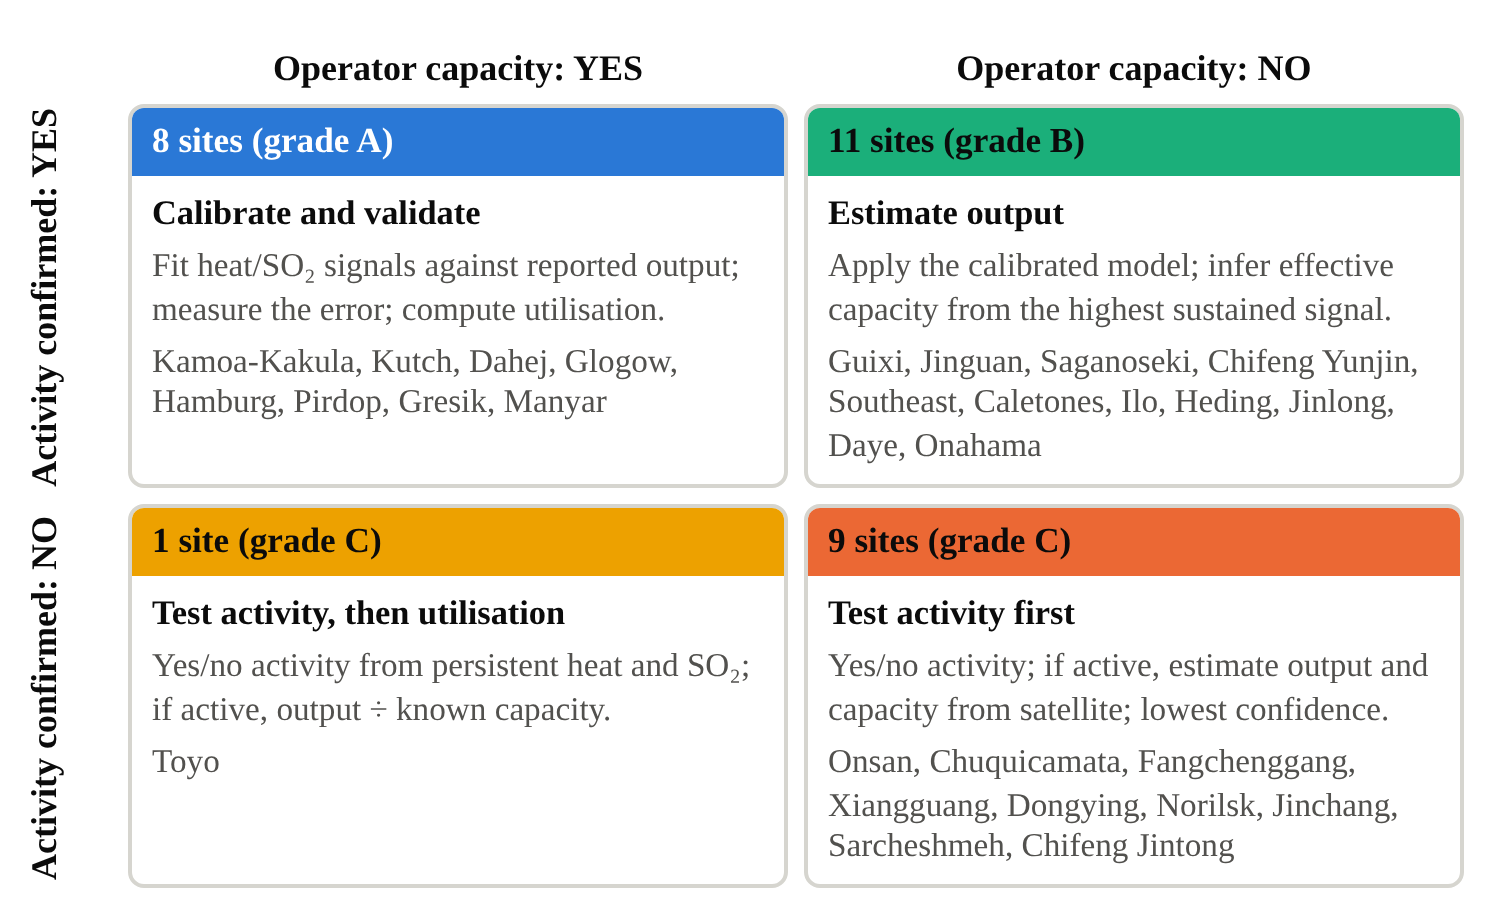
\includegraphics[width=0.7\textwidth,height=\textheight]{figures/status_quad.png}
\caption{Four site statuses and the test strategy for each.}
\end{figure}

The first two rows are the A and B grades; the last two split grade C by
whether a capacity figure exists. Chuquicamata, absent from Codelco's
2026 smelter pages, is the first activity test case.

\textbf{Excluded large smelters.} Altonorte (Chile) stopped in March
2025 for furnace problems and no restart was found
(\href{https://news.metal.com/newscontent/103306296/Glencores-Altonorte-Smelter-Extends-Maintenance-Plan-Raising-Copper-Supply-Concerns}{SMM}).
Ventanas (Chile) closed in 2023 and Paipote (Chile) has been idle since
February 2024
(\href{https://wiki.krisyotam.com/content/wikipedia_en_all_nopic_2026-03/List_of_copper_smelters_in_Chile}{Wikipedia
list}). Potrerillos (Chile) was suspended in 2026 after a structural
failure
(\href{https://www.bcinsight.crugroup.com/2026/07/13/chiles-lawmakers-to-investigate-codelco/}{CRU}).
Guangxi Nanguo and Daye's 400 kt Yangxin Hongsheng line were reported
suspended in December 2024
(\href{https://www.argusmedia.com/en/news-and-insights/latest-market-news/2642686-viewpoint-cu-smelting-capacity-to-outpace-mining}{Argus}).
Glencore's Mount Isa (Australia) has been under closure review since
2025, outcome unconfirmed
(\href{https://www.mining.com/glencore-workers-brace-for-layoffs-on-mount-isa-looming-shutdown/}{MINING.COM}).
These shutdowns fall inside the 2018-present backfill and serve as
validation events (requirement 5).

\textbf{Share of world supply.} The registry holds about 11.7 Mt/yr,
around 47\% of the 24.7 Mt/yr active capacity counted by SAVANT in 2024
{[}13{]}; the share is probably lower now, as about 2.8 Mt/yr of new
capacity was expected in 2025 {[}14{]}. Against 2025 world output, 11.7
Mt equals 40\% of refined production (29.0 Mt) and 51\% of mine
production (23.0 Mt) {[}15{]}. Actual output is lower than capacity:
Argus expected utilisation near 70\% in 2025 {[}14{]}, which puts these
sites at roughly 28\% of world refined copper. Refined production also
includes SX-EW and scrap refining, which no smelter observation
captures.

\hypertarget{methods-and-implementation}{%
\section{4. Methods and
Implementation}\label{methods-and-implementation}}

The ingestion layer (requirement 2) and the geolocation of the registry
were implemented on 4 November 2026 in the Python package
\texttt{orbitcu}
(\href{https://github.com/RobinDemClu/OrbitCu---SWE/pull/1}{pull request
\#1}). Sentinel-2, Landsat 8/9 and VIIRS run end to end. Sentinel-5P and
ERA5 are implemented and unit-tested but could not yet be run (Section
5). The method is documented in \texttt{docs/ingestion.md} and the
prototype numbers in \texttt{docs/prototype\_results.md}.

\hypertarget{code-layout}{%
\subsection{4.1 Code layout}\label{code-layout}}

\begin{longtable}[]{@{}
  >{\raggedright\arraybackslash}p{(\columnwidth - 2\tabcolsep) * \real{0.5000}}
  >{\raggedright\arraybackslash}p{(\columnwidth - 2\tabcolsep) * \real{0.5000}}@{}}
\toprule\noalign{}
\begin{minipage}[b]{\linewidth}\raggedright
Module
\end{minipage} & \begin{minipage}[b]{\linewidth}\raggedright
Role
\end{minipage} \\
\midrule\noalign{}
\endhead
\bottomrule\noalign{}
\endlastfoot
\texttt{sites.py} & Site model: furnace point, 3 × 3 km thermal box, 50
km SO₂ disc, all built in the local UTM zone \\
\texttt{geolocate.py} & Persistent-cluster geolocation from VIIRS,
Sentinel-2 thermal anomaly index (TAI) hot pixels \\
\texttt{activity\_check.py} & Monthly VIIRS detection days and an active
/ intermittent / inactive verdict \\
\texttt{ingest/pit.py} & Point-in-time availability rules \\
\texttt{ingest/optical.py} & Sentinel-2 L2A and Landsat 8/9 Collection-2
L2 clips \\
\texttt{ingest/firms.py} & NASA FIRMS VIIRS client (SP archive, then
NRT) \\
\texttt{ingest/s5p.py} & Sentinel-5P TROPOMI SO₂ pixels inside the 50 km
disc \\
\texttt{ingest/era5.py} & ERA5 10 m and 100 m wind and boundary-layer
height \\
\texttt{cli.py} & \texttt{orbitcu\ firms\ /\ optical\ /\ s5p\ /\ era5}
commands \\
\end{longtable}

There are 18 unit tests, and none of them needs the network.

\hypertarget{areas-of-interest}{%
\subsection{4.2 Areas of interest}\label{areas-of-interest}}

Each site is reduced to one furnace point. The thermal AOI is a square
of half-side 1.5 km and is used for Sentinel-2, Landsat and VIIRS. The
SO₂ AOI is a 50 km disc and is used for TROPOMI pixels and the ERA5 box.
Both are computed in metres in the site's UTM zone, so that boxes have
the same size at 69° N (Norilsk) and at the equator.

\hypertarget{geolocation-of-the-29-smelters}{%
\subsection{4.3 Geolocation of the 29
smelters}\label{geolocation-of-the-29-smelters}}

No gazetteer was reachable from the build environment (OpenStreetMap,
Wikipedia and Wikidata are blocked), so every coordinate was derived
from satellite data, starting from a town- or address-level prior. (1)
One year of VIIRS S-NPP standard-processing detections (2025-08-01 to
2026-07-31) was downloaded within ±25 km of the prior {[}17{]}. (2)
Detections were clustered greedily (densest 500 m cell, then all points
within 1.5 km, then the median position), and each cluster was described
by its number of detection days, its share of FIRMS type-2 ``static land
source'' detections, and its distance to the prior. Persistent
industrial heat sources are well documented in VIIRS data {[}19, 20{]}.
(3) Each candidate was checked on the 10 clearest 2026 Sentinel-2 scenes
with the thermal anomaly index TAI = (B12 − B11) / B8A \textgreater{}
0.45 {[}21{]}. (4) The analyst then chose a location and graded it.
\textbf{High} (10 sites) means one dominant static cluster within about
6 km of the prior. \textbf{Medium} (5 sites) means a clear cluster with
a competing industrial source nearby, or one more than 10 km from a
county-level prior. \textbf{Low} (14 sites) means several candidate
plants (Tongling, Chifeng, Huangshi), no cluster at all (Japan, Gresik,
Kamoa-Kakula), or only a town-level prior. Steel works, refineries and
power plants are also persistent heat sources, so low-confidence sites
carry \texttt{needs\_review\ =\ True} and must be confirmed on a map
before the backfill. The result is
\texttt{data/registry/smelter\_sites.csv}.

On its own, the TAI test turned out to be too permissive in humid and
urban scenes: bright roofs pass the threshold on isolated scenes. It is
therefore used only as a persistence criterion (pixels hot on at least
25 \% of clear scenes), and never as a single-scene detector.

\hypertarget{ingestion}{%
\subsection{4.4 Ingestion}\label{ingestion}}

\begin{longtable}[]{@{}
  >{\raggedright\arraybackslash}p{(\columnwidth - 6\tabcolsep) * \real{0.2500}}
  >{\raggedright\arraybackslash}p{(\columnwidth - 6\tabcolsep) * \real{0.2500}}
  >{\raggedright\arraybackslash}p{(\columnwidth - 6\tabcolsep) * \real{0.2500}}
  >{\raggedright\arraybackslash}p{(\columnwidth - 6\tabcolsep) * \real{0.2500}}@{}}
\toprule\noalign{}
\begin{minipage}[b]{\linewidth}\raggedright
Source
\end{minipage} & \begin{minipage}[b]{\linewidth}\raggedright
Access
\end{minipage} & \begin{minipage}[b]{\linewidth}\raggedright
Stored
\end{minipage} & \begin{minipage}[b]{\linewidth}\raggedright
available\_at
\end{minipage} \\
\midrule\noalign{}
\endhead
\bottomrule\noalign{}
\endlastfoot
Sentinel-2 L2A & STAC search, then the data API \texttt{item/bbox} crop
in the native UTM grid & B8A, B11, B12, SCL clip &
\texttt{s2:generation\_time} \\
Landsat 8/9 C2 L2 & Same as Sentinel-2 & nir08, swir16, swir22, lwir11,
qa\_pixel clip & STAC \texttt{created} \\
VIIRS S-NPP, NOAA-20, NOAA-21 & FIRMS area API, in 5-day chunks: SP up
to its last date, then NRT & All detections in the thermal box &
Acquisition + 3 h \\
Sentinel-5P SO₂ & STAC search, then HTTP byte-range reads of the netCDF
& Pixels in the 50 km disc, with qa\_value & Processing time from the
file name \\
ERA5 & CDS API, monthly per site, on the 0.25° grid & u/v at 10 m and
100 m, boundary-layer height & Valid time + 5 days (ERA5T) \\
\end{longtable}

Only the AOI is ever transferred: the Planetary Computer data API crops
the Cloud-Optimised GeoTIFFs on the server, which is about 90 kB per
Sentinel-2 scene instead of about 1 GB per tile {[}16{]}. Per scene, the
manifest stores the provider's scene cloud cover and the AOI-level
cloud, shadow and no-data fractions. These come from the Sentinel-2 SCL
classes (8, 9, 10 for cloud, 3 for shadow, 0 for no data) or from the
Landsat QA\_PIXEL bits (1, 2, 3 for cloud, 4 for shadow, 0 for fill).
Scenes whose footprint does not fully contain the AOI are dropped, and
duplicate acquisitions on overlapping MGRS tiles or WRS-2 rows are
removed.

\hypertarget{point-in-time-metadata}{%
\subsection{4.5 Point-in-time metadata}\label{point-in-time-metadata}}

Every record carries \texttt{acquired\_at}, \texttt{available\_at},
\texttt{pit\_basis} and \texttt{ingested\_at}, all in UTC. The backtest
may only use records with \texttt{available\_at} ≤ decision time
(\texttt{pit.usable}). The provider's processing timestamp is used when
it exists and is not earlier than the acquisition. Otherwise a
conservative latency applies: FIRMS NRT 3 h, S5P NRTI 3 h and OFFL 5
days, ERA5T 5 days. Known approximations are documented in the code.
Planetary Computer Sentinel-2 is the reprocessed baseline 05.xx, so its
generation time can be later than the original release, which errs on
the safe side. FIRMS SP detections are stamped with the NRT latency,
although the NRT and SP detection sets differ slightly. ERA5T is
replaced by final ERA5 after 2--3 months.

\hypertarget{prototype-glogow-hamburg-kamoa-kakula-nov-2025-oct-2026}{%
\subsection{4.6 Prototype: Glogow, Hamburg, Kamoa-Kakula (Nov 2025 --
Oct
2026)}\label{prototype-glogow-hamburg-kamoa-kakula-nov-2025-oct-2026}}

\begin{longtable}[]{@{}
  >{\raggedright\arraybackslash}p{(\columnwidth - 10\tabcolsep) * \real{0.1667}}
  >{\raggedright\arraybackslash}p{(\columnwidth - 10\tabcolsep) * \real{0.1667}}
  >{\raggedright\arraybackslash}p{(\columnwidth - 10\tabcolsep) * \real{0.1667}}
  >{\raggedright\arraybackslash}p{(\columnwidth - 10\tabcolsep) * \real{0.1667}}
  >{\raggedright\arraybackslash}p{(\columnwidth - 10\tabcolsep) * \real{0.1667}}
  >{\raggedright\arraybackslash}p{(\columnwidth - 10\tabcolsep) * \real{0.1667}}@{}}
\toprule\noalign{}
\begin{minipage}[b]{\linewidth}\raggedright
Site
\end{minipage} & \begin{minipage}[b]{\linewidth}\raggedright
Geolocation
\end{minipage} & \begin{minipage}[b]{\linewidth}\raggedright
Sentinel-2 scenes (clear)
\end{minipage} & \begin{minipage}[b]{\linewidth}\raggedright
Clear scenes with ≥ 3 hot pixels
\end{minipage} & \begin{minipage}[b]{\linewidth}\raggedright
Landsat scenes (clear)
\end{minipage} & \begin{minipage}[b]{\linewidth}\raggedright
VIIRS detections (days)
\end{minipage} \\
\midrule\noalign{}
\endhead
\bottomrule\noalign{}
\endlastfoot
Glogow & high & 203 (62) & 59 / 62 & 44 (10) & 2001 (276) \\
Hamburg & medium & 100 (27) & 21 / 27 & 71 (21) & 580 (169) \\
Kamoa-Kakula & low & 102 (53) & 8 / 53 & 56 (34) & 61 (19) \\
\end{longtable}

All 576 optical clips (89 MB) were fetched with no failure after
retries. The median lag between acquisition and availability is 4--5 h
for Sentinel-2, 19--32 days for Landsat Collection-2 L2, and 3 h for
VIIRS. Glogow is the reference case: the furnace area is hot on 95 \% of
clear Sentinel-2 scenes and is seen by VIIRS on 276 days of the year.
Hamburg is clearly active at the chosen point. At Kamoa-Kakula, the
smelter started in late 2025 and its location is still a prior, so the
box probably misses the furnace; it must be located by hand.

\hypertarget{satellite-check-of-the-grade-c-sites}{%
\subsection{4.7 Satellite check of the grade-C
sites}\label{satellite-check-of-the-grade-c-sites}}

For the 10 sites without a dated operator confirmation, we counted the
distinct VIIRS detection days per month within 1.5 km (S-NPP; SP up to
July 2026, NRT afterwards) and checked Sentinel-2 hot-pixel persistence.
Eight sites are active in VIIRS: Sarcheshmeh (294 detection days from
November 2025 to October 2026), Chuquicamata (237, near zero in
June--July 2026), Xiangguang (235), Norilsk Copper Plant (206),
Fangchenggang (183), Dongying (173), Chifeng Jintong (159) and Jinchang
(158). Onsan (48 days) and Toyo (0) are weak in VIIRS but show
persistent Sentinel-2 hot pixels on 10/10 and 8/10 clear scenes, so they
are classed as likely active. For a low-confidence location, ``active''
only means that an industrial heat source at that point is running. The
results are in \texttt{data/registry/c\_site\_activity\_check.csv}.

\hypertarget{interactive-status-map-first-dashboard-view}{%
\subsection{4.8 Interactive status map (first dashboard
view)}\label{interactive-status-map-first-dashboard-view}}

A self-contained HTML map shows the 29 smelters at their furnace points,
sized by capacity, with an activity status that the reader can follow
month by month (\texttt{statusmap.py}). For each site and each month
from January 2025 to October 2026, the generator counts the distinct
days with a VIIRS S-NPP detection within 1.5 km of the furnace (SP
archive, then NRT for August--October 2026). The site's typical level is
the median of these counts over the months with at least one detection,
so a long outage does not lower the reference; a site detected in fewer
than 3 months gets no typical level. In the page, the reader picks a
month and a window of 1, 3 or 12 months. The detection rate over that
window is compared with the typical level: \textbf{active} at 50 \% of
it or more, \textbf{reduced} below 50 \% but above zero, \textbf{no heat
detected} at zero, and \textbf{signal too weak} when there is no typical
level or it is under 2 days per month, since VIIRS cannot then support a
conclusion (Kamoa-Kakula, Toyo, Onahama and PT Smelting in October
2026). Low-confidence locations are drawn with a dashed outline. The
base map is Natural Earth 1:50m, embedded as TopoJSON and drawn with d3,
so the page needs no tile server. This status is a transparent first
proxy for the detection and fusion stages (requirements 3 and 4): it
uses one sensor, ignores cloud cover, and therefore under-reads sites in
persistently cloudy months.

\hypertarget{development-environment-and-implementation-plan}{%
\subsection{4.9 Development environment and implementation
plan}\label{development-environment-and-implementation-plan}}

On 5 November 2026 the proposal was extended with the development
environment and a specification of every requirement (Word file
\texttt{OrbitCu\_Proposal\_Requirements\_v2.docx}). The pipeline runs as
Linux containers on Kubernetes, written in Python 3.12, and is used
through a Plotly Dash web dashboard. Development happens on Windows 11
laptops through WSL 2 and Docker; the reference workstation is Windows
11 Pro (build 26200) with 32 GB of RAM.

\begin{longtable}[]{@{}
  >{\raggedright\arraybackslash}p{(\columnwidth - 4\tabcolsep) * \real{0.3333}}
  >{\raggedright\arraybackslash}p{(\columnwidth - 4\tabcolsep) * \real{0.3333}}
  >{\raggedright\arraybackslash}p{(\columnwidth - 4\tabcolsep) * \real{0.3333}}@{}}
\toprule\noalign{}
\begin{minipage}[b]{\linewidth}\raggedright
Layer
\end{minipage} & \begin{minipage}[b]{\linewidth}\raggedright
Choice
\end{minipage} & \begin{minipage}[b]{\linewidth}\raggedright
Reason
\end{minipage} \\
\midrule\noalign{}
\endhead
\bottomrule\noalign{}
\endlastfoot
Orchestration & Argo Workflows and Argo Events on Kubernetes (kind
locally, Azure AKS in West Europe as the cloud option) & Backfill =
thousands of small (site, month, sensor) jobs, retried independently;
AKS sits in the same Azure region as the Planetary Computer, so no
egress \\
Storage & Downloaded image clips, one score per image, and daily results
(probabilities, indices, official figures), stored as files on the
laptop or on Azure storage & Every row keeps \texttt{acquired\_at},
\texttt{available\_at}, \texttt{ingested\_at}, so any date can be
replayed \\
Tracking & MLflow & Parameters and metrics of detection, fusion, nowcast
and backtest runs \\
Market data & LSEG Workspace via the LSEG Data Library for Python &
Individual futures contracts (COMEX HG, LME, SHFE) needed for rolls;
licence already held by a team member, so raw data stay private \\
\end{longtable}

\textbf{Cost.} The build costs nothing: data and software are free, LSEG
Workspace is already available to a team member, the team uses its own
laptops, and the optional Azure deployment is covered by the free Azure
for Students plan (\$100 of credit per member).

\textbf{Planned algorithms.} Thermal score: Sentinel-2/Landsat hot
pixels with TAI \textgreater{} 0.45 (Section 4.7) and VIIRS night
detections with their fire radiative power {[}20{]}. SO₂: TROPOMI
columns with qa\_value ≥ 0.5, rotated into the ERA5 wind {[}23{]} and
fitted with an exponentially modified Gaussian {[}22{]}, cross-checked
with flux divergence {[}8{]}, {[}24{]}. Fusion: a two-state hidden
Markov model per site, forward-filtered so that only past data enter the
daily P(active), with missing observations left out of the likelihood
{[}25{]}; indices weight P(active) by registry capacity. Nowcast: bridge
regression of monthly output growth on month-to-date index means,
trained on first releases only {[}26{]}. Backtest: walk-forward folds,
roll five business days before first notice, one tick of slippage per
side, deflated Sharpe ratio to correct for the number of configurations
tried {[}27{]}.

\hypertarget{difficulties-and-decisions}{%
\section{5. Difficulties and
Decisions}\label{difficulties-and-decisions}}

\begin{longtable}[]{@{}
  >{\raggedright\arraybackslash}p{(\columnwidth - 4\tabcolsep) * \real{0.3333}}
  >{\raggedright\arraybackslash}p{(\columnwidth - 4\tabcolsep) * \real{0.3333}}
  >{\raggedright\arraybackslash}p{(\columnwidth - 4\tabcolsep) * \real{0.3333}}@{}}
\toprule\noalign{}
\begin{minipage}[b]{\linewidth}\raggedright
Date
\end{minipage} & \begin{minipage}[b]{\linewidth}\raggedright
Issue
\end{minipage} & \begin{minipage}[b]{\linewidth}\raggedright
Decision
\end{minipage} \\
\midrule\noalign{}
\endhead
\bottomrule\noalign{}
\endlastfoot
2026-11-04 & No free, current, plant-level smelter capacity table
exists; sources mix years and bases (blister, anode, cathode) & Cite one
source per site, record basis and confidence, and harmonise capacities
before computing indices \\
2026-11-04 & The first seed list (Statista) ranked refineries, which
have no satellite signature & Discarded; registry restricted to primary
smelters active in 2026 \\
2026-11-04 & Several large smelters are idle or under review
(Potrerillos, Nanguo, Mount Isa, Manyar, PT Smelting) & Exclude
permanently closed or suspended sites; keep restarting sites with a
status flag; use closures as validation events \\
2026-11-04 & Operator-level output figures do not prove that a given
site is running & Every site checked against its operator's own
documents and graded A, B or C; C sites get satellite confirmation
first \\
2026-11-04 & Operators rarely publish site capacity, and several Chinese
operator websites and NICICO refuse automated access & Keep secondary
capacity figures where needed, flagged as such; broker reports used only
as labelled secondary sources \\
2026-11-04 & Operator documents contradicted two registry rows (Nadezhda
is a nickel plant; the Chifeng plant of Yunnan Copper is Chifeng Yunjin)
& Rows corrected to the site the operator reports \\
2026-11-04 & Catalogue APIs answer, but the files are served from other
hosts (Azure Blob Storage for Sentinel-5P, an ECMWF object store for
CDS) that the cloud network allow-list blocks & Use the Planetary
Computer pixel cut-out API for Sentinel-2 and Landsat; Sentinel-5P and
ERA5 stay blocked until those hosts are allowed \\
2026-11-04 & The CDS rejects ERA5 requests until the account accepts the
dataset licence & Licence accepted by Rob on the project account; test
request queued \\
2026-11-04 & FIRMS quota (5,000 transactions per 10 minutes, 5 days per
area request) was reached while geolocating the 29 sites & Throttle
requests and resume automatically; use small boxes around each site \\
2026-11-04 & No gazetteer (OpenStreetMap, Wikipedia, Wikidata) is
reachable from the cloud environment, so plant coordinates cannot be
looked up or cited from a web source & Locate plants from satellite data
(VIIRS persistent clusters plus Sentinel-2 TAI) and grade each location;
14 low-confidence sites are flagged for a manual map check \\
2026-11-04 & Several cities host more than one heat source (Tongling,
Chifeng, Huangshi, Hamburg), and single-scene TAI flags bright roofs in
humid or urban scenes & Use hot-pixel persistence across scenes rather
than single scenes; keep the plant-to-cluster mapping as low confidence
until confirmed \\
2026-11-04 & Sentinel-2 tiles and Landsat rows overlap; some STAC items
only partly cover a site & Keep only items whose footprint contains the
AOI, and remove duplicate acquisitions \\
2026-11-04 & The FIRMS key-status counter stays near 5,000 while
requests are accepted again, so a throttle that waited for it to drop
blocked the download for 15 minutes & Do not gate on the counter; back
off 60 s and retry only when FIRMS actually refuses a request (HTTP
400) \\
\end{longtable}

\hypertarget{references-part-ii}{%
\section{References (Part II)}\label{references-part-ii}}

{[}1{]} Earth-i, ``Metals Smelting Insight.''
https://earthi.space/services/savant-metals-smelting-insight/

{[}2{]} Earth-i, ``Earth-i announces launch of the SAVANT Global Copper
Smelting Index,'' Oct.~8, 2019. https://earthi.space/?p=5293

{[}3{]} MINING.COM, ``Satellites to monitor copper supply from space,''
Oct.~9, 2019.
https://www.mining.com/satellites-to-monitor-copper-supply-from-space/

{[}4{]} Shanghai Metals Market, ``Satellite-based monitoring firm state
primary smelter activity remains strong,'' Nov.~18, 2025.
https://news.metal.com/newscontent/103625040

{[}5{]} Climate TRACE, ``Conversations with the Coalition:
TransitionZero,'' Jul.~23, 2024.
https://climatetrace.org/news/conversations-with-the-coalition-transitionzero

{[}6{]} F. Massimetti et al., ``Volcanic hot-spot detection using
SENTINEL-2,'' Remote Sens., vol.~12, no. 5, 820, 2020,
doi:10.3390/rs12050820.

{[}7{]} V. E. Fioletov et al., ``A global catalogue of large SO₂ sources
and emissions derived from the Ozone Monitoring Instrument,'' Atmos.
Chem. Phys., vol.~16, pp.~11497--11519, 2016,
doi:10.5194/acp-16-11497-2016.

{[}8{]} G. Kuhlmann et al., ``The ddeq Python library for point source
quantification from remote sensing images (version 1.0),'' Geosci. Model
Dev., vol.~17, pp.~4773--4789, 2024, doi:10.5194/gmd-17-4773-2024.

{[}9{]} D. P. Finch and P. I. Palmer, ``Towards automated near-real-time
global monitoring of atmospheric SO₂ plumes from satellite data using
U-Net segmentation,'' Atmos. Meas. Tech., vol.~19, pp.~4049--4064, 2026,
doi:10.5194/amt-19-4049-2026.

{[}10{]} Microsoft, ``Planetary Computer data catalog.''
https://planetarycomputer.microsoft.com/catalog

{[}11{]} Statista (source: ICSG), ``Leading copper refineries worldwide
in 2025, based on capacity,'' April 2025.
https://www.statista.com/statistics/1180215/global-leading-copper-refineries-by-capacity/

{[}12{]} International Copper Study Group, ``The World Copper Factbook
2020,'' Top 20 copper smelters by capacity, p.~20.
https://internationalcopper.org/wp-content/uploads/2021/01/2020\_10\_13\_ICSG\_Factbook\_2020.pdf

{[}13{]} Earth-i, ``Earth-i releases 2024 SAVANT Copper Database
update,'' Aug.~16, 2024. https://earthi.space/?p=16261

{[}14{]} Argus Media, ``Viewpoint: Cu smelting capacity to outpace
mining,'' Dec.~30, 2024.
https://www.argusmedia.com/en/news-and-insights/latest-market-news/2642686-viewpoint-cu-smelting-capacity-to-outpace-mining

{[}15{]} U.S. Geological Survey, ``Mineral Commodity Summaries 2026:
Copper,'' Feb.~2026.
https://pubs.usgs.gov/periodicals/mcs2026/mcs2026-copper.pdf

{[}16{]} Microsoft Planetary Computer, STAC API collections
sentinel-2-l2a, landsat-c2-l2 and sentinel-5p-l2-netcdf (accessed
Nov.~4, 2026).
https://planetarycomputer.microsoft.com/api/stac/v1/collections

{[}17{]} NASA LANCE, ``Fire Information for Resource Management System
(FIRMS)'' and ``FIRMS API: area'' (accessed Nov.~4, 2026).
https://firms.modaps.eosdis.nasa.gov/api/area/

{[}18{]} Copernicus Climate Change Service, ``ERA5 hourly data on single
levels from 1940 to present,'' Climate Data Store (accessed Nov.~4,
2026).
https://cds.climate.copernicus.eu/datasets/reanalysis-era5-single-levels

{[}19{]} Y. Liu et al., ``Identifying industrial heat sources using
time-series of the VIIRS Nightfire product with an object-oriented
approach,'' Remote Sens. Environ., vol.~204, pp.~347--365, 2018.

{[}20{]} W. Schroeder et al., ``The New VIIRS 375 m active fire
detection data product: Algorithm description and initial assessment,''
Remote Sens. Environ., vol.~143, pp.~85--96, 2014.

{[}21{]} F. Marchese et al., ``A multi-channel algorithm for mapping
volcanic thermal anomalies by means of Sentinel-2 MSI and Landsat-8 OLI
data,'' Remote Sens., vol.~11, no. 23, 2876, 2019.

{[}22{]} V. Fioletov et al., ``Anthropogenic and volcanic point source
SO₂ emissions derived from TROPOMI on board Sentinel-5 Precursor: first
results,'' Atmos. Chem. Phys., vol.~20, pp.~5591--5607, 2020.

{[}23{]} H. Hersbach et al., ``The ERA5 global reanalysis,'' Q. J. R.
Meteorol. Soc., vol.~146, pp.~1999--2049, 2020.

{[}24{]} S. Beirle et al., ``Pinpointing nitrogen oxide emissions from
space,'' Sci. Adv., vol.~5, no. 11, eaax9800, 2019, doi:
10.1126/sciadv.aax9800.

{[}25{]} L. R. Rabiner, ``A tutorial on hidden Markov models and
selected applications in speech recognition,'' Proc. IEEE, vol.~77, no.
2, pp.~257--286, 1989, doi: 10.1109/5.18626.

{[}26{]} D. Giannone, L. Reichlin, and D. Small, ``Nowcasting: The
real-time informational content of macroeconomic data,'' J. Monetary
Econ., vol.~55, no. 4, pp.~665--676, 2008, doi:
10.1016/j.jmoneco.2008.05.010.

{[}27{]} D. H. Bailey and M. López de Prado, ``The deflated Sharpe
ratio: Correcting for selection bias, backtest overfitting, and
non-normality,'' J. Portfolio Manage., vol.~40, no. 5, pp.~94--107,
2014, doi: 10.3905/jpm.2014.40.5.094.

\end{document}
